\documentclass[conference]{IEEEtran}
\IEEEoverridecommandlockouts
\usepackage{cite}
\usepackage{amsmath,amssymb,amsfonts}
\usepackage{algorithmic}
\usepackage{graphicx}
\usepackage{textcomp}
\usepackage{xcolor}
\def\BibTeX{{\rm B\kern-.05em{\sc i\kern-.025em b}\kern-.08em
    T\kern-.1667em\lower.7ex\hbox{E}\kern-.125emX}}
\begin{document}

\title{HyperPS: A Hypervisor Monitoring Approach Based on Privilege Separation}

%1\textsuperscript{st}
\author{\IEEEauthorblockN {Kunli Lin,Wenqing Liu}
\IEEEauthorblockA{\textit{Institute of Information Engineering, Chinese Academy of Sciences} \\
\textit{School of Cyber Security, University of Chinese Academy of Sciences}\\
%\{xxx\}@iie.ac.cn}%
\{linkunli,liuwenqing\}@iie.ac.cn}
}
\maketitle

\begin{abstract}

%Privilege separation has long been considered as a fundamental principle in software design to mitigate the potential damage of a security attack. Much effort has been given to develop various privilege separation schemes where a monolithic OS or hypervisor is divided into two privilege domains where one domain is logically more privileged than the other even if they both run at an identical processor privilege level.

%In monitic operating system (OS), both kernel code and hypervisor code is in the same address space, security mechanisms are shared by kernel and hypervisor, an error of system software can be exploited to destroy the whole system. 
%Once compromising the hypervisor which provides resource allocation and management for guest virtual machines (VMs), adversaries can easily access other customers' sensitive data of VMs. Therefore, it is essential to adopt some security mechanisms to guarantee the integrity of hypervisor and monitor it. In addition, privilege separation has long been considered as a fundamental principle in software design to mitigate the potential damage of a security attack for monolithic OS or hypervisor. It can create a trusted execution environment to isolate the key function modules.
%%, transplant the shared-environment feature designed in monitic OS or hypervisor.
% However, previous efforts employ microhypervisor which is not convenient for cloud providers to adopt widely. Or they employ a new software relying on higher privilege level.
\iffalse
In monistic operating system, an error of system software can be exploit to destroy the whole system. The situation becomes much more severe in cloud environment, when the kernel and the hypervisor share the same address space. The security of guest Virtual Machines (VMs), both sensitive data and vital code, can no longer be guaranteed, once the hypervisor is compromised. Therefore, it is essential to deploy some security approaches to secure VMs, regardless of the hypervisor is safe or not. Some efforts such as microhypervisor, have been put forward to address this problem, however, they are not convenient for current commercial cloud providers. Or some works employ a new software relying on higher privilege-level.

As malware and attacks increase against 
%virtually every level of privileged software including an OS and a
 hypervisor, we have been motivated to develop a prototype, named as HyperPS, to realize hypervisor monitoring based on true privilege separation. HyperPS does not rely on microhypervisor or a more privileged software. 
The key of HyperPS is that it decouples the interaction functions between VM and the hypervisor by monitoring VMCS and EPT. As a result, HyperPS monitors the interaction, monitors memory mapping of VM, and resists system information leakage attack.
We have implemented a prototype for KVM hypervisor on x86 platform with multiple VMs running Linux. KVM with HyperPS can be applied to current commercial cloud computing industry with portability. The security analysis shows that this approach can provide effective monitoring against attacks, and the performance evaluation confirms the efficiency of HyperPS.
\fi
In monolithic operating system (OS), any error of system software can be exploit to destroy the whole system. The situation becomes much more severe in cloud environment, when the kernel and the hypervisor share the same address space. The security of guest Virtual Machines (VMs), both sensitive data and vital code, can no longer be guaranteed, once the hypervisor is compromised. Therefore, it is essential to deploy some security approaches to secure VMs, regardless of the hypervisor is safe or not. Some approaches propose microhypervisor reducing attack surface, or a new software requiring a higher privilege level than hypervisor.

In this paper, we propose a novel approach, named HyperPS, which separates the fundamental and crucial privilege into a new trusted environment in order to monitor hypervisor. A pivotal condition for HyperPS is that hypervisor must not be allowed to manipulate any security-sensitive system resources, such as page tables, system control registers, interaction between VM and hypervisor as well as VM memory mapping. Besides, HyperPS proposes a trusted environment which does not rely on any higher privilege than any privileged software including the OS and the hypervisor. We have implemented a prototype for KVM hypervisor on x86 platform with multiple VMs running Linux. KVM with HyperPS can be applied to current commercial cloud computing industry with portability. The security analysis shows that this approach can provide effective monitoring against attacks, and the performance evaluation confirms the efficiency of HyperPS.

\end{abstract}

\begin{IEEEkeywords}
Virtualization, Hypervisor Monitoring, Hypervisor Security, Cloud Computing
\end{IEEEkeywords}

\section{Introduction}

%A variety of system software such as an operating system (OS) and virtual machine monitor (hypervisor) has a 
%monolithic design, which integrates its core services into one huge code base, thereby encompassing them all in a single address space and executing them in the same processor privilege level (i.e., ring 0 and VMX-root modes in Intel x86 or svc and hyp modes in ARM). 
%
%As more and more functionalities are added into OS and the hypervisor, the code bases of commodity system have been increased to be larger. Larger code base  size consequently increases the risk of having security vulnerabilities. 
%Take the hypervisor as an example, from 2004 to now, there are 130 vulnerabilities about KVM.
%%Some of them (e.g., CVE-2018-1087)\ref{} shows high-risk vulnerabilities that can lead to privilege raising behavior and comprehensive compromised hypervisor.
% Because hypervisor possesses the highest privilege in the cloud environment, attackers who compromise hypervisor can harm the whole cloud infrastructure and endanger data and computation in the system.
%Therefore, vulnerabilities residing in a fraction of system software can be easily exploited to subvert other parts of or the whole system.
%
%%Privilege separation stemming from the work of Schroeder\cite{zhaobudao} has been considered as a fundamental principle in software design that can remove such a security concern.
%
%%系统中的代码越来越多,攻击面越大,同权限的系统组件,一旦被攻击会对系统中的其余部分造成影响,所以需要做权限分离。
%
%Attackers who aim to manipulate system resources and take over the control of a system have been able to compromise each and every level of system software. An exploit of any part of the kernel allows complete access to all memory and resources on the system. Consequently, commodity OSes have been susceptible to a range of kernel malware and memory corruption attacks.
%In order to reduce the threat to other components or the whole system caused by attackers, enforce this security principle in the design, current researchers achieve privilege separation by creating more privileged software or introducing microkernel, microhypervisor.


%In general, the Trusted Computing Base (TCB) of a typical hypervisor has to be big enough to handle resource allocation and hardware peripheral virtualization. 
In general, the larger code base of a typical hypervisor consequently increases the risk of having security vulnerabilities.
Furthermore, successful VM escape attacks, as well as the emerging hypervisor rootkits, greatly make threats for VMs.
In light of these attacks, there is a pressing need to investigate effective ways to monitor the hypervisor. 
% makes commodity hypervisors struggle with security problems.
%Therefore, commodity hypervisors are already big enough to struggle with security problems.
% A recent study of the National Vulnerability Database indicates that in the last three years, there are 26 security vulnerabilities identified in Xen and 18 in VMware ESX. 
%Some CVE vulnerabilities can be directly exploited to execute arbitrary code in the hypervisor. 
%Furthermore, successful VM escape attacks, as well as the emerging hypervisor rootkits, greatly make threats for VMs.
%exacerbate the current situation. 
%In light of these attacks, there is a pressing need to investigate effective ways to monitor the hypervisor. 
%One natural but challenging approach is to formally separate the critical capability from the hypervisor. 
In addition to larger code base of hypervisor, monolithic system design can also increase the risk of being attacked.
%A variety of system software such as an OS and hypervisor has a monolithic design, which integrates its core services into one huge code base, thereby encompassing them all in a single address space and executing them in the same processor privilege level (i.e., ring 0 and VMX-root modes in Intel x86 or svc and hyp modes in ARM).
Software with monolithic design integrates core services into one huge code base, thereby encompassing them all in a single address space and executing them in the same processor privilege level (i.e., ring 0 and VMX-root modes in Intel x86 or svc and hyp modes in ARM).
% Attackers who aim to manipulate system resources and take over the control of a system are  able to compromise each and every level of system software.
OS kernels define and store access control policies in main memory, hypervisor controls VM memory allocation and interaction data access between the VM and the hypervisor where any code executing within the hypervisor can modify.
An exploit of any part of the hypervisor allows complete access to all memory and critical resource. %Consequently, commodity OSes have been susceptible to a range of malware and memory corruption attacks.
Privilege separation stemming from the work of Schroeder\cite{zhaobudao} has been considered as a fundamental principle that can separate the critical capability from the hypervisor and remove such a security concern.

In order to reduce the threat to other components or the whole system caused by attackers, and enforce this security principle in the design, current researchers achieve privilege separation by introducing microhypervisor or creating more privileged software.


%\textbf{Hardware}
%Some efforts (SecureME\cite{Chhabra2011SecureME}, Bastion\cite{Champagne2010Scalable} and Iso-x\cite{Evtyushkin2015Iso}) rely on 
%customized underlying hardware to provide fine-grained protection for VM or in-VM process. 
%Iso-X provides isolation for security-critical pieces of an application by introducing additional hardware and changes to OS. It controls memory access by introducing ISA instructions. 
%Bastion uses modified microprocessor hardware based on FPGA to protect the storage and runtime memory state of enhanced hypervisor against both software and hardware attacks. So that it provides hardware-protected environment and protection for security-critical OS and application modules in an untrusted software stack.
%Different hardware platforms provide different hardware mechanisms,such as Intel's Software Guard Extensions (SGX) \cite{WuLLCZG18}. 
%%and AMD's Secure Memory Encryption (SME).
%SGX provides protection for pieces of application logic inside encrypted enclave memory against malicious OS. However, it is limited to protect a relatively small portion
%of memory, and the developers have to mostly reconstruct the protected software or build it from scratch. Therefore it is nontrivial for SGX to protect large-scale software like the entire VM. 
\textbf{Microhypervisor}
By abandoning the monolithic design and modularizing core services, the microhypervisor design achieves privilege separation.
% The microkernel is a thin kernel\cite{Klein2009SeL4} which can prevent damage of a fraction of the OS kernel from spreading across the whole kernel.
Trustvisor\cite{J2010TrustVisor} uses a microhypervisor to provide privilege separation and verify security sensitive workloads, eventually prevents damage of a fraction of the hypervisor from spreading across the whole system. Nova\cite{Steinberg2010NOVA} uses microhypervisor to provide privilege separation and memory protection for the virtualization layer. Nevertheless, this design has been deemed unrealistic for cloud providers in that it usually necessitates reorganization of the current system software architecture. 

%\textbf{Reorganization System}
%%一些工作通过将物理资源访问权限进行分离,从而避免被攻击的内核或者虚拟机监控器的恶意访问。这些工作主要是给每个虚拟机预分配固定的物理核和内存来管理对敏感信息的访问权限。
%Some works  (NoHype\cite{NoHype} and TrustOSV\cite{TrustOSV}) avoids malicious access to the attacked kernel or virtual machine monitor by separating the access privilege of physical resources. These tasks are mainly to pre-allocate a fixed physical core and memory to each VM to manage access to sensitive data. NoHype removes most of virtualization functions from hypervisor while retaining the key features enabled by virtualization and prepares packup for each VM. More recent techniques to split existing commodity operating systems into multiple protection domains using page protections incuring high overhead.

\textbf{A Higher Privilege-level Software }
In order to mitigate the hazard caused by the hypervisor, plenty of solutions propose and introduce a higher privilege-level software than the original hypervisor.
% To isolate kernel, researchers turn their focus onto an additional security layer in the system, such as a hypervisor\cite{Wang2015SecPod}, SMM of Intel\cite{Wang2010HyperCheck}, or TrustZone of ARM\cite{Sprobes}, which has a higher privilege over kernel. A clear advantage of this design is that it does not entail substantial modifications in the current software architecture. Some of them are customized for hardware features.
Nested virtualization  \cite{Ben2007The}, \cite{Zhang2011CloudVisor} is one of the representative approaches to isolate hypervisor, which provides a higher privilege-level execution environment to run the monitor securely. 
The turtles project \cite{Ben2007The} and CloudVisor \cite{Zhang2011CloudVisor} are examples of systems that propose nested virtualization idea to achieve isolation for protected resources. 
%Especially, CloudVisor uses nested virtualization to decouple resource management into the nested hypervisor to protect VMs.
%Also, the mandatory involvement of more privileged software in its design usually entails frequent switching between different privilege levels for the security enforcement, which is a definite cause of the overall system performance degradation.

%
%For the system software with monolithic design, such as an operating system (OS) and hypervisor, this coexist environment is the entirety of the kernel and hypervisor, including potentially buggy device drivers and so on, forms a single large trusted computing base (TCB) for all applications on the system.
%The impact of it is that any exploit of any part of this system can allow complete access to all VM memory and resources on the system.
%Therefore, to address these problems, we propose HyperPS which divides the kernel or hypervisor into two worlds, Normal World and HyperPS World. HyperPS can isolate the memory region of HyperPS World from Normal World in the same privilege-level.
%除了上述提到的权限分离技术,
%当前的系统往往是一体化的,攻击者可以攻击系统中的内核或者hypervisor从而对整个系统进行攻击。已经有一些学者在x86平台上的通过对权限分离对内核实施了完整性保护。也有一些学者针对ARM体系架构上实现了对hypervisor和内核的内外部域权限分离。但是这些方法大部分只是实现了内外域的权限分离,并没有实现对hypervisor的安全监控。

%%%%%%%%%%%
%记得改内容 直接翻译的 不准确
%Current commodity systems are often monolithic, and attackers can attack the system's kernel or hypervisor to compromise the entire system. Some researches have implemented integrity protection on the x86 platform by separating privilege. Some have also implemented the privilege separation for hypervisor and kernel based on ARM architecture. However, most of these methods only realize the privilege separation, and do not realize the security monitoring of hypervisor.


%我们提出的HyperPS原型,提供了一个基于特权分离的内部域的hypervisor监控,不依赖额外的硬件,也不依赖更高特权级的软件层。该原型可以针对大部分硬件处理器,对系统进行小改动,对云平台提供商相对友好。
In this paper, we introduce a novel prototype, named HyperPS, to implement hypervisor monitoring based on privilege separation in every level of privileged software without relying on a higher privileged software or microhypervisor. It has applicability for multi-platforms (x86, mips and so on), few modifications for original hypervisor, and practicability for cloud providers.
We take x86 architecture as an example.
%设计的核心是通过特权分离的方法创建隔离的域空间,在该空间中对关键的数据结构实施监控。HyperPS监控了虚拟机与宿主机交互的唯一关键数据结构vmcs,和虚拟机地址映射中使用的数据结构EPT,避免恶意的攻击造成整个系统的compromised。vmcs的重要性能和EPT的重要性讲述,参看原论文。

The key of the design is to create an isolated space by separating privileges, in which HyperPS can monitor runtime hypervisor. 
HyperPS ensures that the hypervisor never disables protection-mechanism (e.g., DEP, SMEP) by efficiently decoupling updating privilege of critical registers into HyperPS World.
Hypervisor monitoring is executed by monitoring key data structures including Extended Page Tables (EPT) and Virtual Machine Control Structure (VMCS),
%It monitors VMCS, which is used to record system status during VM interacts with the hypervisor, and EPT, used in the address mapping of VM, 
so as to avoid malicious attacks causing the whole system compromised. VMCS is used in VMX operation to manage the behavior of VMs as well as transitions between the VM and the hypervisor. Thus, the modification of content of VMCS, especially the Guest-state filed and VM-execution control field, may cause unpredictable consequences. EPT contains the mapping relationship from Guest Physical Address (GPA) to Host Physical Address (HPA). Given the great importance of the data structures mentioned above, HyperPS isolates them beyond access from compromised parts of system.



Our prototype introduces 3K SLOC (Source Lines of Code) to hypervisor monitoring and 270 SLOC modifications of the hypervisor.
% VM monitoring reduces the attack surface of the hypervisor, and the memory isolation among hypervisor and VMs is significantly guaranteed. 
The experimental results show trivial performance overhead and independence on multi-platforms for runtime hypervisor monitoring. 


Our contributions are as follows:
\begin{itemize}
%\item{An introduction of a novel technique, HyperPS, which can implement privilege separation in a variety of system software with different processor privilege levels, such as kernel and a hypervisor.}



\item{A practical event-driven hypervisor monitoring approach based on privilege separation in a variety of system software with hypervisor processor privilege level.}%without any extra hardware or softwares on more privileged level.}
\item{A non-bypassable protection approach for VMCS and EPT which can ensure the security of interaction between VM and hypervisor.}
\item{A prototype based on KVM and x86 architecture with trivial performance overhead, high security and hardware independence.}% portability.}
\end{itemize}

The rest of this paper is organized as follows. Section \ref{background} describes background. Section \ref{sec:threat} discusses our threat model and assumption. Section \ref{sec:design} elaborates on the design and implementation of HyperPS on x86 platform. Section \ref{sec:evaluation} gives the evaluation of security and performance. Section \ref{sec:related} compares HyperPS with previous work. At last, Section \ref{sec:conclusion} gives the conclusion.

%
%背景知识:
%VMCS 
%之前一些文章中有仔细描述
%
%再讲一下虚拟机退出
%
%两大段
%
%
%EPT
%虚拟机的地址映射一把需要两套页表,一套用于自身操作系统,将客户机虚拟机地址转换为…… 之前的文章可能写了,copy 一下,加快时间写。


\section{Background}\label{background}

\subsection{VMCS}
Virtualization technique imports two kinds of operation mode, Root and Non-root mode. % which processor runs on. 
%When the processor runs in non-root mode, VM runs on the virtual CPU (vCPU), and when the processor runs in root mode, the hypervisor runs on the vCPU. 
%Switching between the two modes, named context switching, means switching between VM and the hypervisor running on the vCPU. 
%it is called context switch.
%虚拟化技术引入了两种模式,两种模式的切换意味着系统之间的切换。
%为了更好地支持CPU虚拟化,VT-X技术引入了VMCS结构体,来保存vCPU需要的状态信息,例如根模式和非根模式下特权寄存器的值等。该结构体包含了许多域,记录了客户机信息的客户机域和记录宿主机信息的宿主机域。
To better support CPU virtualization, VMCS structure, a data structure based on hardware, is imported to manage transitions out and into of VMX Non-root mode from VMX Root mode (VM Exit and VM Entry), as well as processor behavior.
This structure is divided into six information fields, including Guest-state filed which records VM information and Host-state filed which records host OS information.
It causes VM Exit that the vCPU switches from root mode to non-root mode. The reverse operation is called VM Entry that transiting from non-root mode to root mode. During these two operations, VMCS is used primarily for vCPU to query and update key CPU information such as system privileged registers.

%The processor will trigger a VM exit and return to root mode, then handle some operations. 
%处理器从根模式切换到非根模式,会引发虚拟机退出,反操作被称为虚拟机及进入。VMCS主要供vCPU在虚拟机退出和进入时查询和更新特权寄存器等关键信息。


%
% 虚拟机退出主要因为客户机有部分敏感指令无法正常执行,需要hypervisor的协助完成敏感执行操作。当虚拟机退出执行完后,需要执行一些VMLAUNCH/VMRESUME指令发起虚拟机进入。一般的虚拟机退出流程如下:
%1)CPU首先将此次VM Exit的原因信息记录到VMCS相应的信息域中,并将CPU状态保存到VMCS客户机状态域中。
%2)CPU将VMCS中hypervisor状态信息读取并加载到自身的CPU中。
%3)CPU读取VMCS中的虚拟机退出原因,从非根模式切换到根模式,并跳转到虚拟机退出处理函数入口执行。
%4)虚拟机退出函数处理结束后,CPU执行VMLAUNCH/VMRESUME执行发起虚拟机进入重新运行客户机。
\subsection{VM Exit/VM Entry}
Intel's VT-X introduces VMX operations, VM Exit and VM Entry. VM Exit is primarily due to that the VM has some sensitive instructions that cannot be performed properly and requires hypervisor's assistance to complete sensitive instruction execution. After VM Exit is finished, CPU needs to execute VMLAUNCH/VMRESUME instruction to initiate VM Entry. The interaction that is triggered by VM Exit process from the VM to hypervisor is as follows. The execution flow of VM Entry is opposite to that of VM Exit.
%The execution process of the interaction is as follows. 

%In traditional system, VM interacts with hypervisor  by VM EXIT/VM ENTRY to request hypervisor to handle 敏感指令引发的陷入events. The execution process of the interaction is as follows. 

1) VM makes interrupt request for VM Exit, and the CPU in non-root mode first records VM Exit reason to the corresponding information filed in VMCS and saves the CPU state to the Guest-state filed of VMCS.
2) The CPU accesses the Host-state filed of VMCS and loads it into CPU.
3) The CPU switches from non-root mode to root mode, reads VM Exit reason in VMCS, and jumps to VM Exit handler function entry.
%4) After the VM Exit handler function is processed, CPU executes VMLAUNCH/VMRESUME instruction to
4) CPU initiates VM Entry and run the VM.




%1) VM switches context and exits to hypervisor. 2) Hypervisor handles the VM exit request events. 3)  Hypervisor executes VM resume instruction to entry VM.


\subsection{Address Translation of VM}
The address translation of VM requests two page tables, guest page table and EPT. Guest page table can finish the translation from guest virtual address (GVA) to GPA. This translation is finished by VM. The translation from GPA to HPA is executed based on EPT by hypervisor.
% EPT technique is based on hardware and managed by hypervisor.
Intel's VT-x provides EPT, which directly supports address translation from GPA to HPA on hardware, greatly reduces the difficulty of memory virtualization and further improves the performance of virtualization.
%is used to support for memory virtualization at processor level and improve virtualization performance. In the meantime, EPT meets the need of translation from guest physical address (GPA) to host physical address (HPA), the real physical memory address. 





%
%威胁模型
%
%自身环境
%关键数据 交互数据vmcs ept


%\begin{figure}
%\centerline{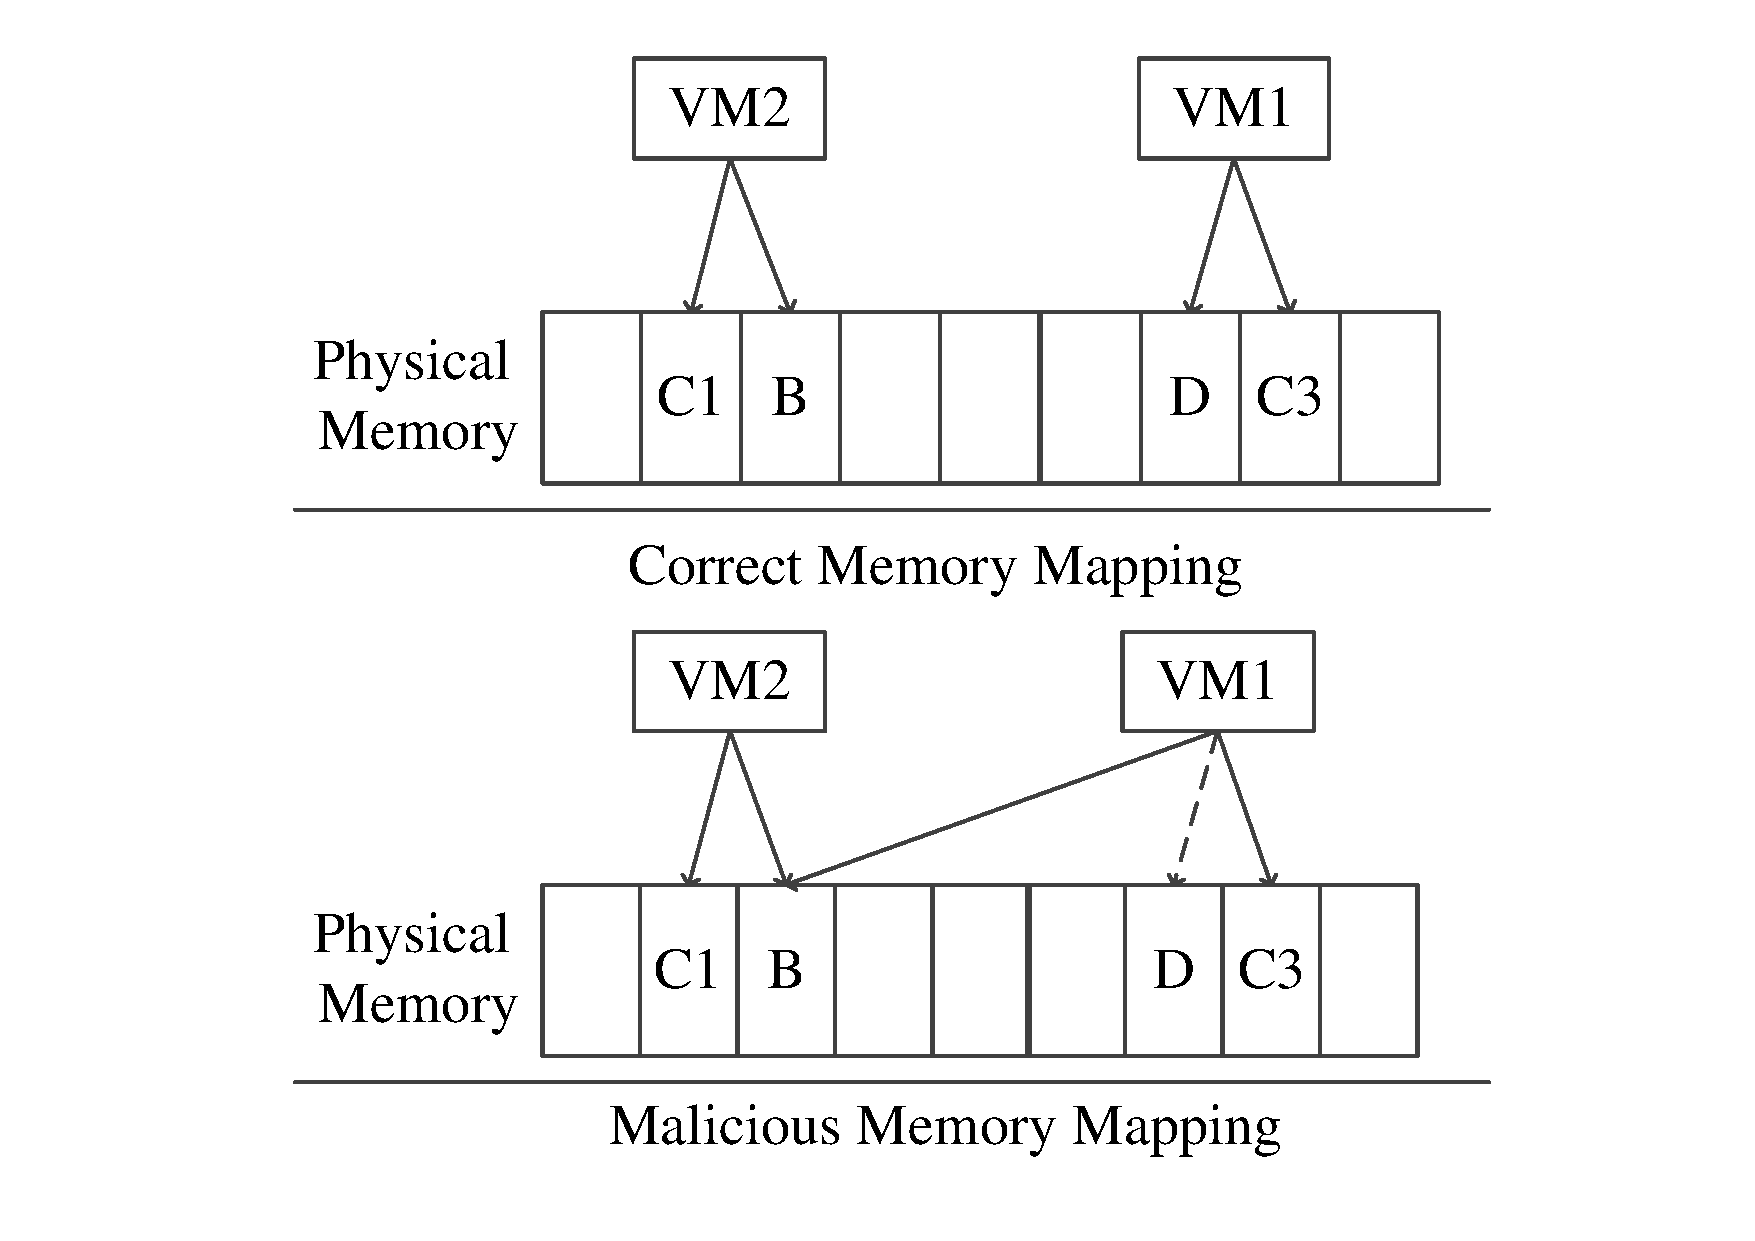
\includegraphics[width=10cm, height=6cm]{pdfvmcs.pdf}}%{pdfvmsm1.jpg}}
%\caption{The execution process of double mapping. } \label{fig0}
%\end{figure}

\begin{figure}
\centerline{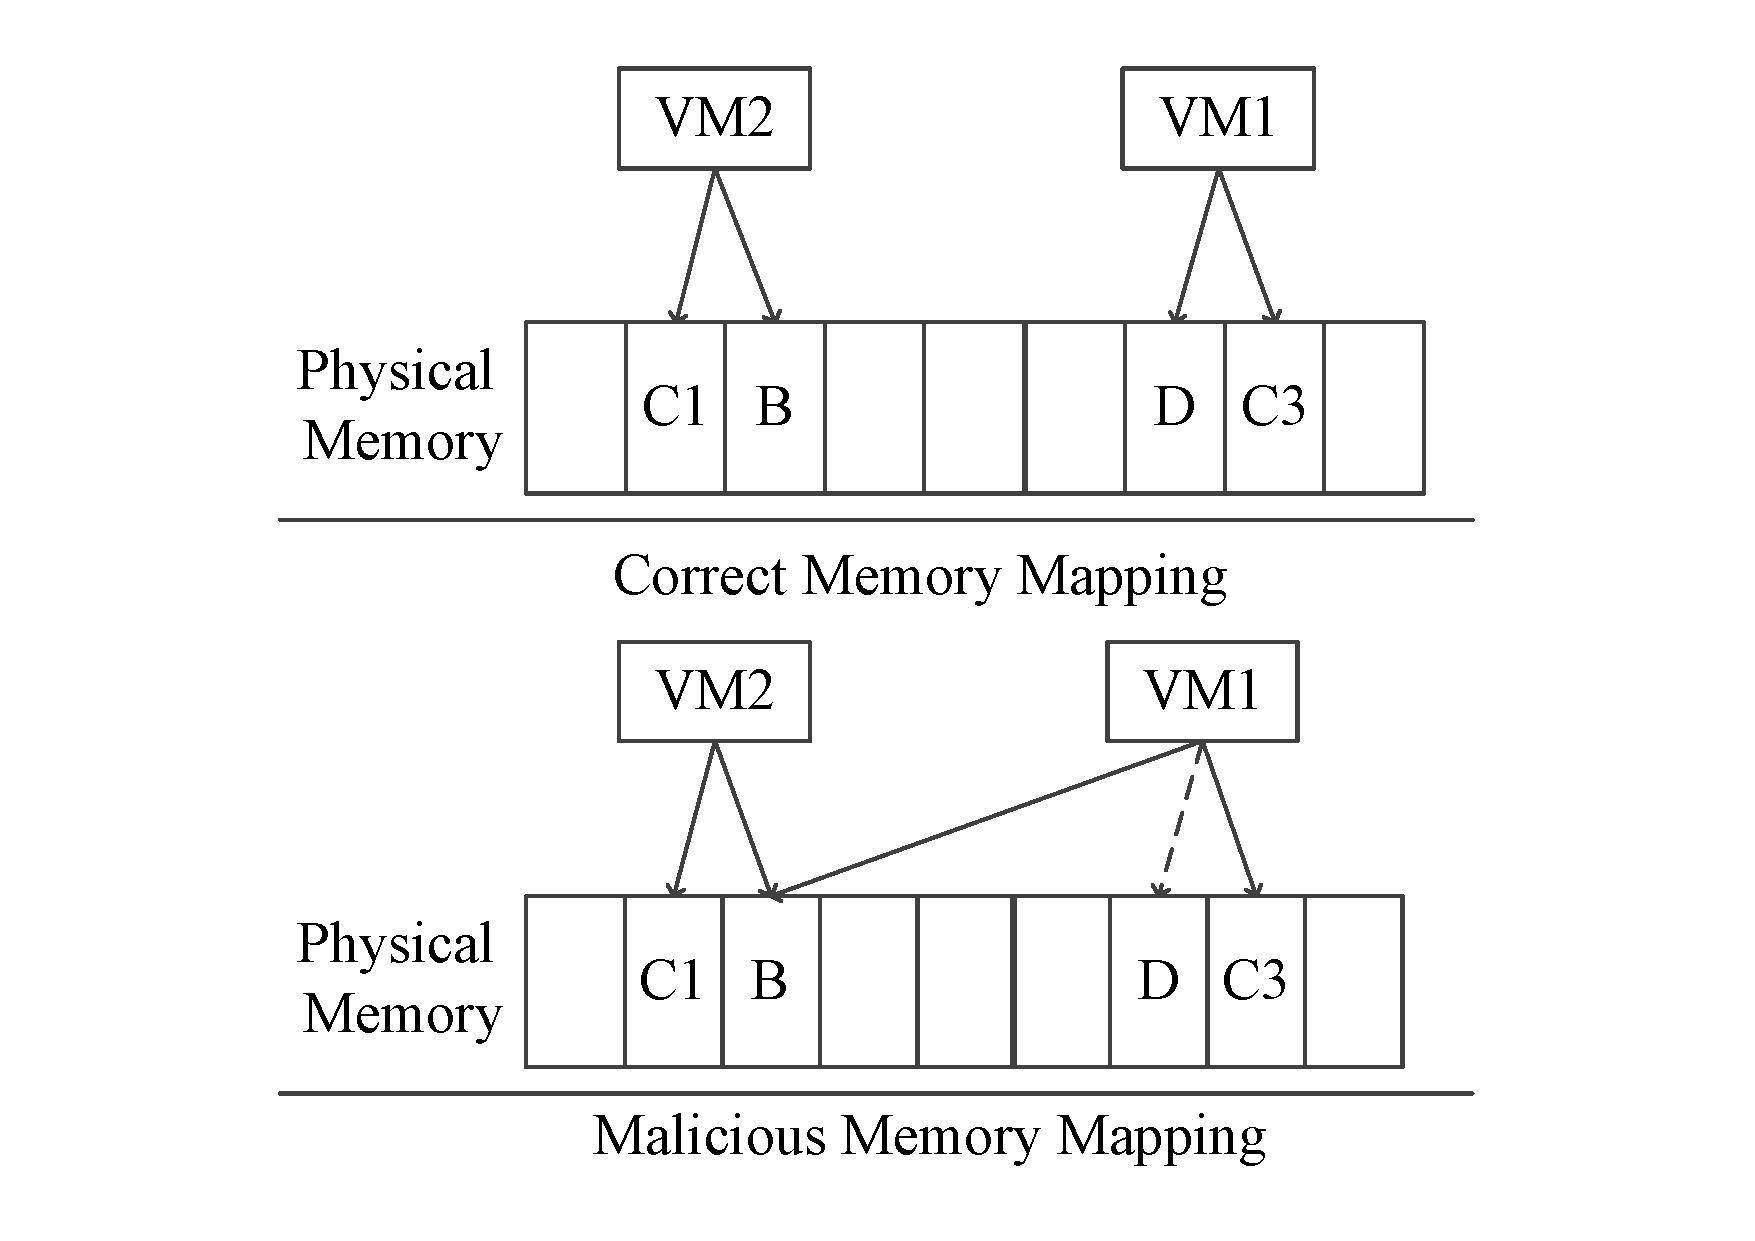
\includegraphics[width=10cm, height=6cm]{pdfvmcs_lkl.pdf}}%{pdfvmsm1.jpg}}
\caption{The execution process of double mapping attack. } \label{fig0}
\end{figure}

\section{Threat Model and Assumption}\label{sec:threat}


\subsection{Threat Model} \label {threat}


%On the one hand, attackers can modify the critical interaction data in the context switching process between VMs and hypervisor. On the other hand, attackers can modify the address mapping of EPT, causing remapping attack and double mapping attack.

We assume that the hypervisor and kernel have been compromised and controlled by the powerful adversary. 
The adversary can turn off kernel security mechanisms, such as DEP,SMEP, inject code, even tamper page table mappings of memory region, and then implement attacks based on two attack paths, compromising critical interaction data and VM address mapping.
First, the adversary can subvert the critical interaction data during the context switching process between VM and the hypervisor. Second, the adversary can tamper values of EPT entry causing memory corruption attacks, such as remapping attack, double mapping attack and disrupting isolation among EPTs.

\paragraph{Modifying the Interaction Data}
For the modification of the critical interaction data during the context switching process, attackers can obtain the address of VMCS
and modify it, such as HOST\_RIP, GUEST\_CR0, EPTP, et al. For example,
modifying the value of privilege register, CR0, can close DEP mechanism, and modifying CR4 can close SMEP mechanism.

\paragraph{Modifying the Address Mapping of EPT}
Modification of EPT entry can result in memory information leakage. There are three attack scenes, double mapping, remapping attack and disrupting isolation among EPTs of VMs.

\textbf{Scene 1.} 
    For double mapping attack, attackers control and compromise a VM, then obtain the privilege of hypervisor through VM escape attack, and maliciously access the VMCS structure to obtain the value of EPT\_Pointer(EPTP). The attack process is as shown in Figure \ref{fig0}. There are two guest VMs, VM1 (attacker) and VM2 (victim). In this way, EPTP of VM1 and EPTP of VM2 are respectively obtained by attackers. Also, for a guest virtual address (GVA) in VM2, named 'A', is mapped to the corresponding real physical address, named 'B'. For VM1, the real physical address corresponding to the guest virtual address 'C' is 'D', then 'D' is modified to be 'B' by modifying the value of the last page item of EPT. At last, 'A' and 'C' are mapped to the real physical address 'B', no address is mapped to 'D'. Then VM1 can access the data of VM2 successfully through accessing 'B', this attack process is called double mapping attack.



\textbf{Scene 2.}
    %For the remapping attack, there are VM1 (attacker) and VM2 (victim).
    In a remapping attack scenario, we assume there are two VMs, VM1, a VM controlled by attackers to attack other VMs, VM2, a victimized VM.
 A physical page (named 'A') used by VM2 is released after it is used and it is released with VM2's content. After 'A' is released, VM1 remaps a GVA (named 'E') to 'A'. By this way, VM1 can access the content on 'A' used by VM2 through 'E', causing information leakage.
Through the analysis of these two kinds of attack models, it is necessary to achieve attack prevention.

\textbf{Scene 3.}
 For disrupting the isolation among EPTs, there is no isolation among current EPTs, and attackers can compromise a VM and hypervisor first, then access memory of VM2 (victim) through VM1 (attacker) through making VM1 load VM2's EPT.
%attackers can 
 %we assume there are two VMs, VM1, a VM controlled by attackers to attack other VMs, VM2, a victimized VM.

%\paragraph{Modifying the Address Mapping of EPT}


\subsection{Assumption}
We propose some assumptions.
First, we assume hardware resources are trusted including processor, buses, BIOS, UEFI and so on, the trusted boot based on hardware can ensure the security and integrity of bootloaders. The Trusted Computing Base (TCB) contains created HyperPS and hardware resources. Second, this paper does not consider denial of service attack (DOS), side channel attack and hardware-based attack, such as cold-boot attack and RowHammer. Third, we assume that there exists no software that runs at a higher privilege level than the hypervisor.

%\begin{figure}
%\centerline{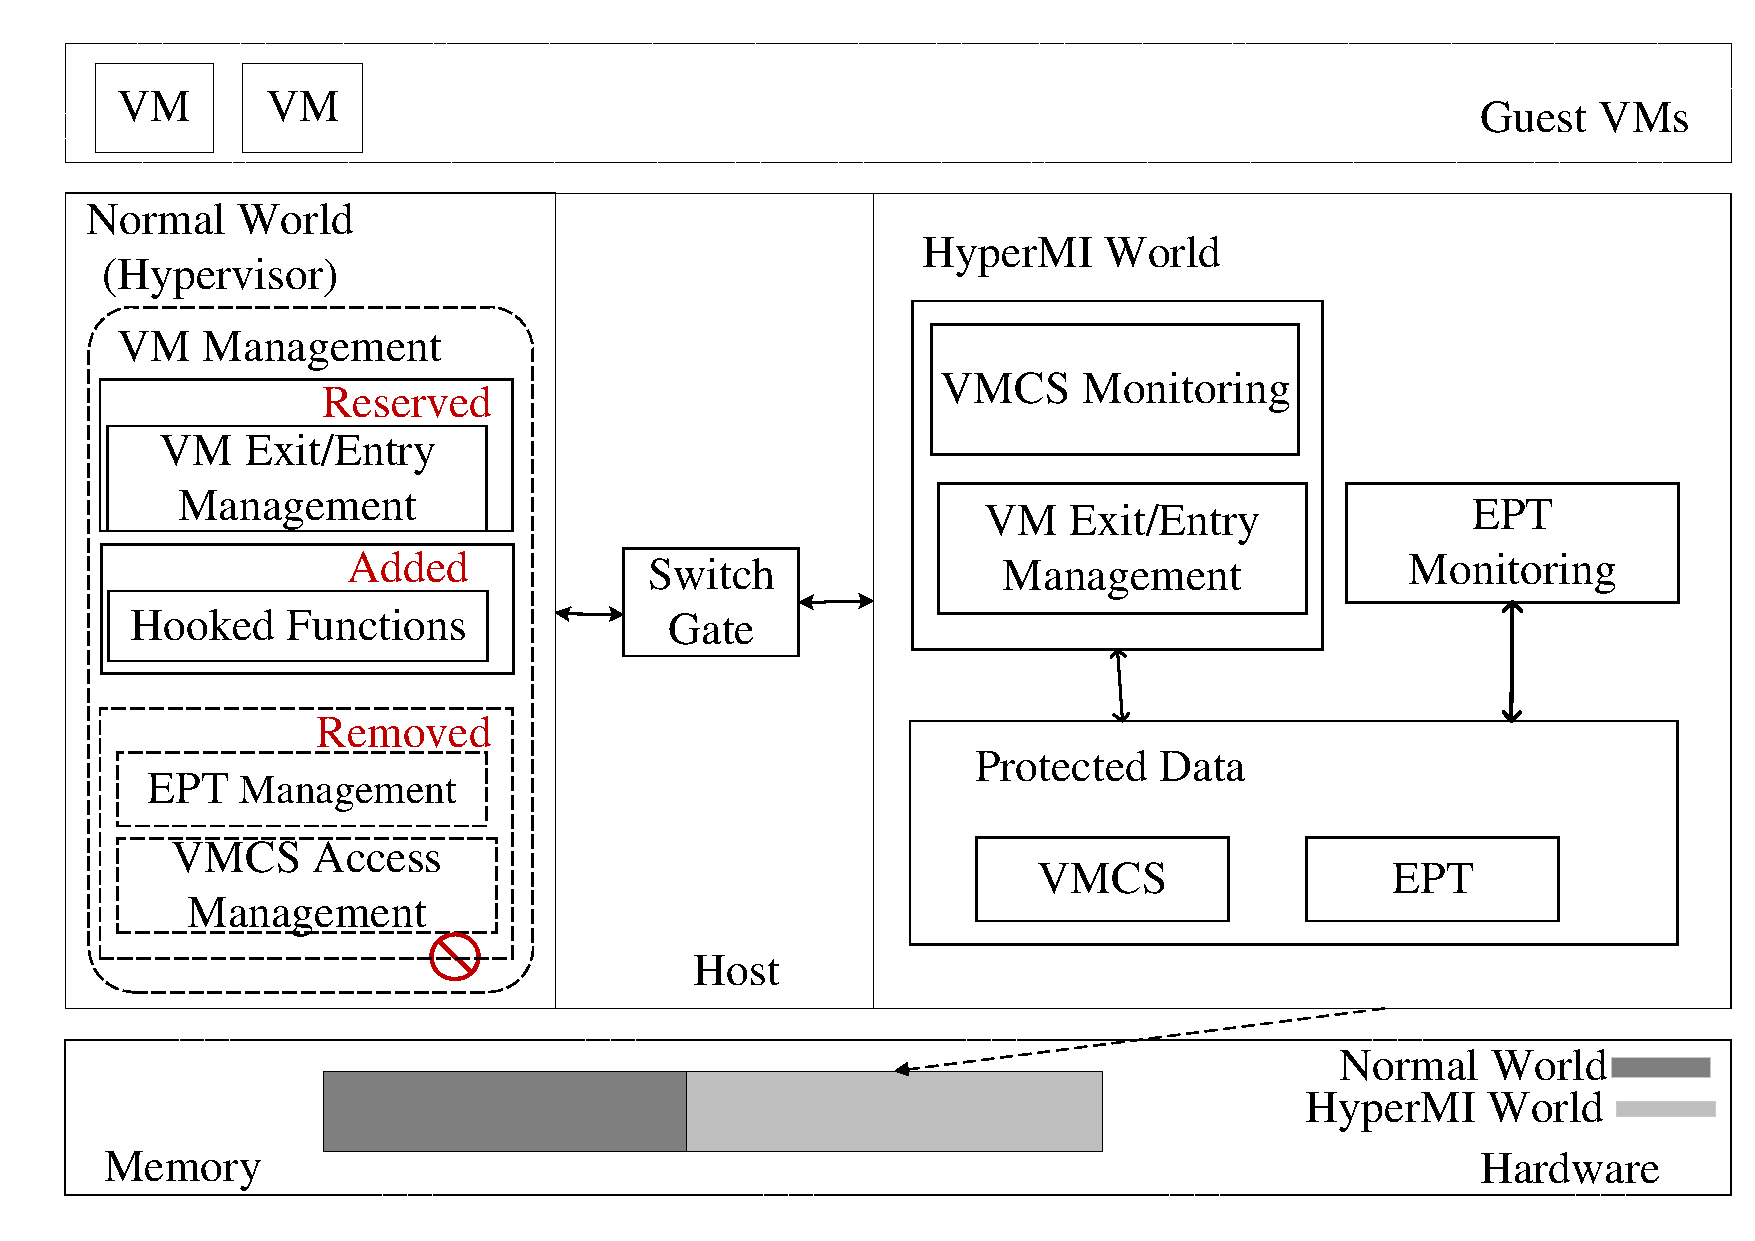
\includegraphics[width=9.5cm, height=7cm]{pdfHyperPSArch.pdf}}%{pdfvmcs1.pdf}}%%{pdfvmsm1.jpg}}
%\caption{The architecture of HyperPS. } \label{fig1}
%\end{figure}


\begin{figure}
\centerline{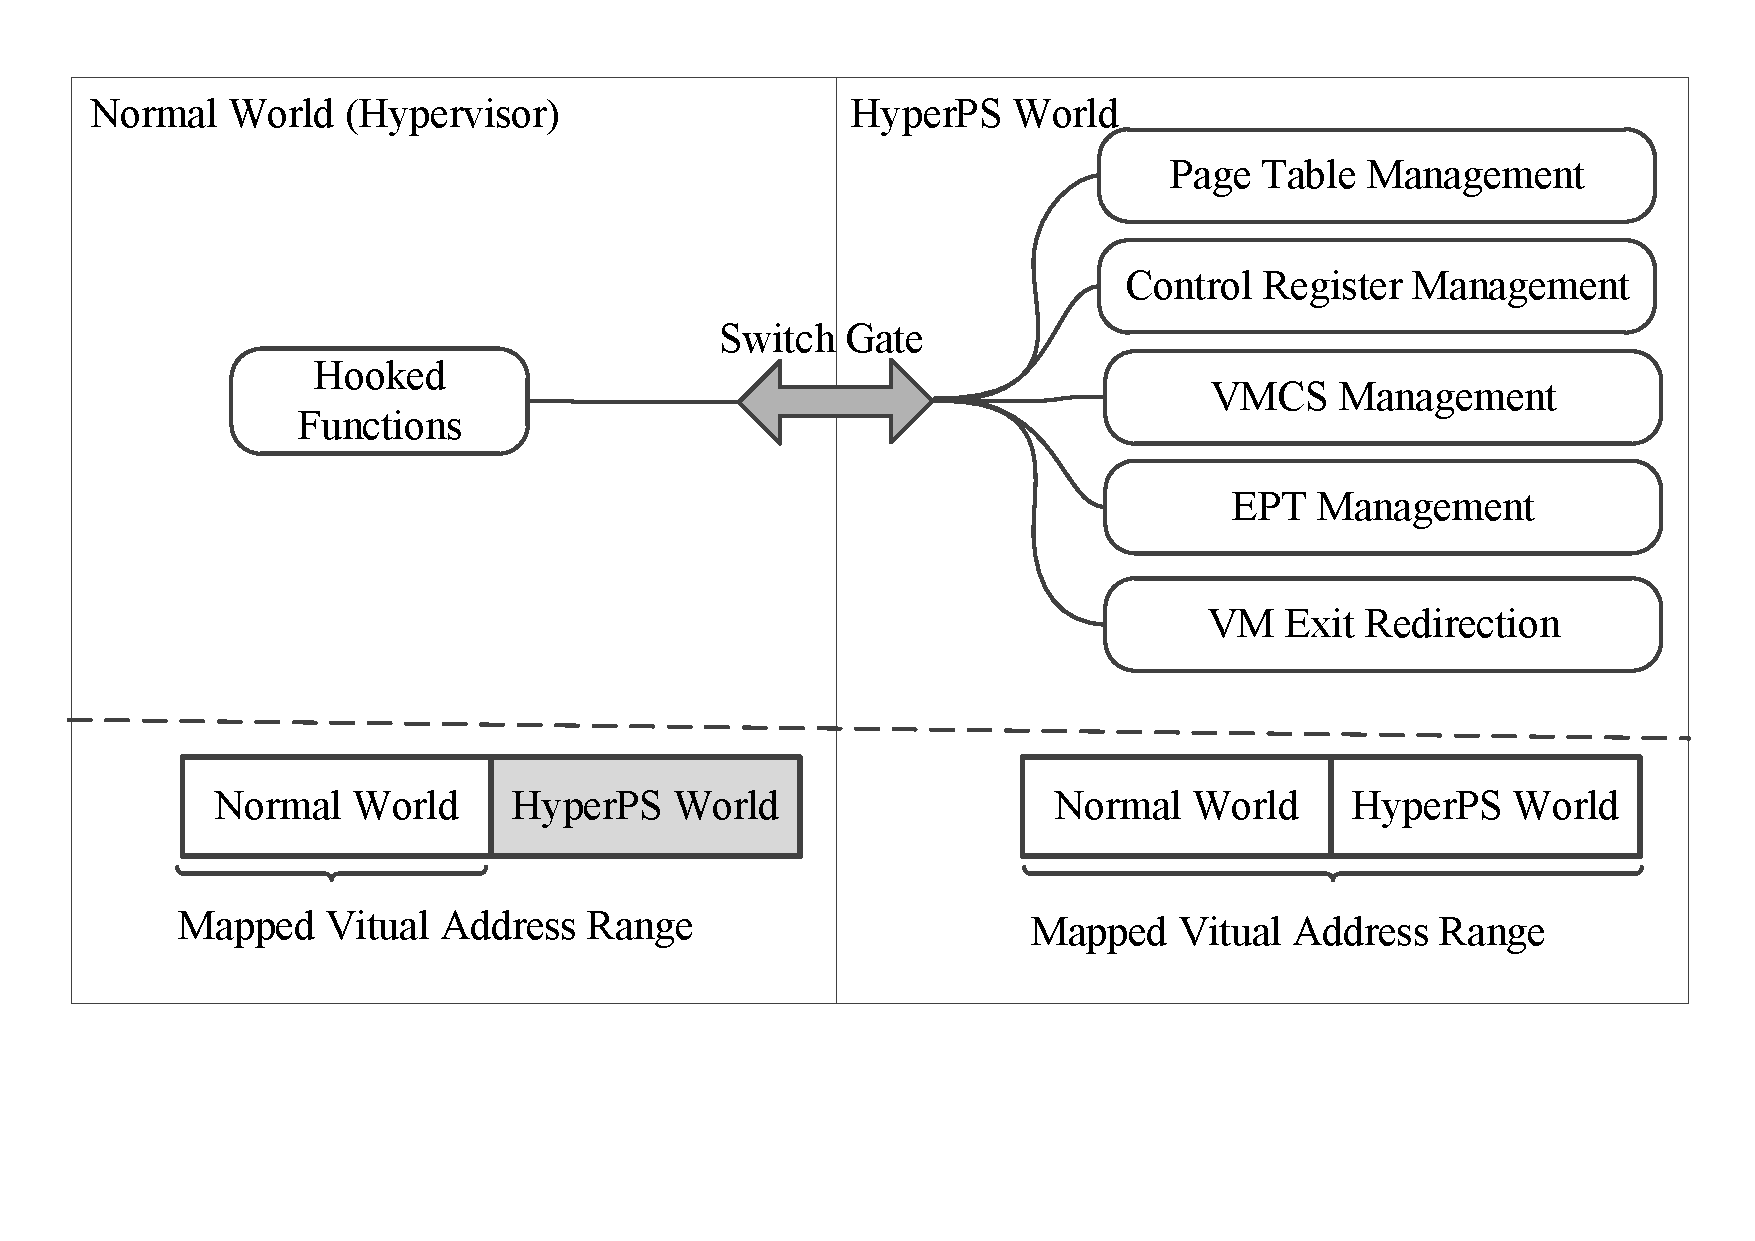
\includegraphics[width=8.5cm, height=5cm]{overview-e.pdf}}%{pdfHyperPSArch_lkl.pdf}}%{pdfvmcs1.pdf}}%%{pdfvmsm1.jpg}}
\setlength{\abovecaptionskip}{3pt}
\setlength{\belowcaptionskip}{2pt}
\caption{The overview of HyperPS. } \label{fig1}
\end{figure}

\section{Design and Implementation}\label{sec:design}

In this section, we present the design and implementation
details of HyperPS, focusing on the two core mechanisms, VMCS and EPT monitoring.



\subsection{Overview} 
%HyperPS is designed to provide a secure isolated execution environment to protect VMs against compromised hypervisor without depending on a higher privilege level software than the hypervisor or hardware.


%Figure \ref{fig1} shows the architecture, the overall system contains three parts: several isolated VMs, hypervisor either in Normal World or in HyperPS word, memory hardware including HyperPS region for HyperPS world and normal region for Normal World.

%The origin hypervisor is divided into two parts: HyperPS domain which security tools can run in and Normal World which hypervisor runs in. Firstly, HyperPS world is used to run security tools, so that these tools running in secure HyperPS world can resist attacks from Normal World. Secondly, operations for EPT and context switching module are deprived from Normal World for security, then are put into HyperPS world, but VM exit handler module is reserved to handle VM exit in Normal World. Thirdly, these two worlds can communicate with each other through the only secure channel, named Switch Gate.
HyperPS is designed to provide a secure domain to provide hypervisor monitoring against attackers without depending on a higher privilege-level software than the hypervisor or microhypervisor. 
Figure \ref{fig1} depicts the overview of HyperPS which creates other secure address spaces based on a set of new page table. It is composed of three parts, Normal World, HyperPS World and Switch Gate. 
A pivotal condition for HyperPS is that Normal World (origin hypervisor) must not be allowed to manipulate any security-sensitive system resources, such as EPT, VMCS, page tables and system control registers.
%that may be used to invalidate hypervisor monitoring. 
To meet this condition, Normal World is deprived of controlling authority over security-sensitive system resources. Therefore, VMCS and EPT are hidden in HyperPS World from Normal World accessing. Instead, Normal World is only allowed to send requests through a specified interface (Switch Gate) to HyperPS World for controlling these resources.
 To assess the security of interaction between hypervisor and VM, VM memory mapping, management on VMCS and EPT, are hooked and trapped to HyperPS World. Page table and control register management is used to guarantee the security of HyperPS World.
VM Exit redirection can balance VM Exit and VMCS management. Upon receiving such a request, HyperPS World determines whether to accept or reject it. More importantly, only virtual address of Normal World is mapped in page table of Normal World while all virtual address of two worlds is mapped in page table of HyperPS World.

%
%\begin{figure}
%\centerline{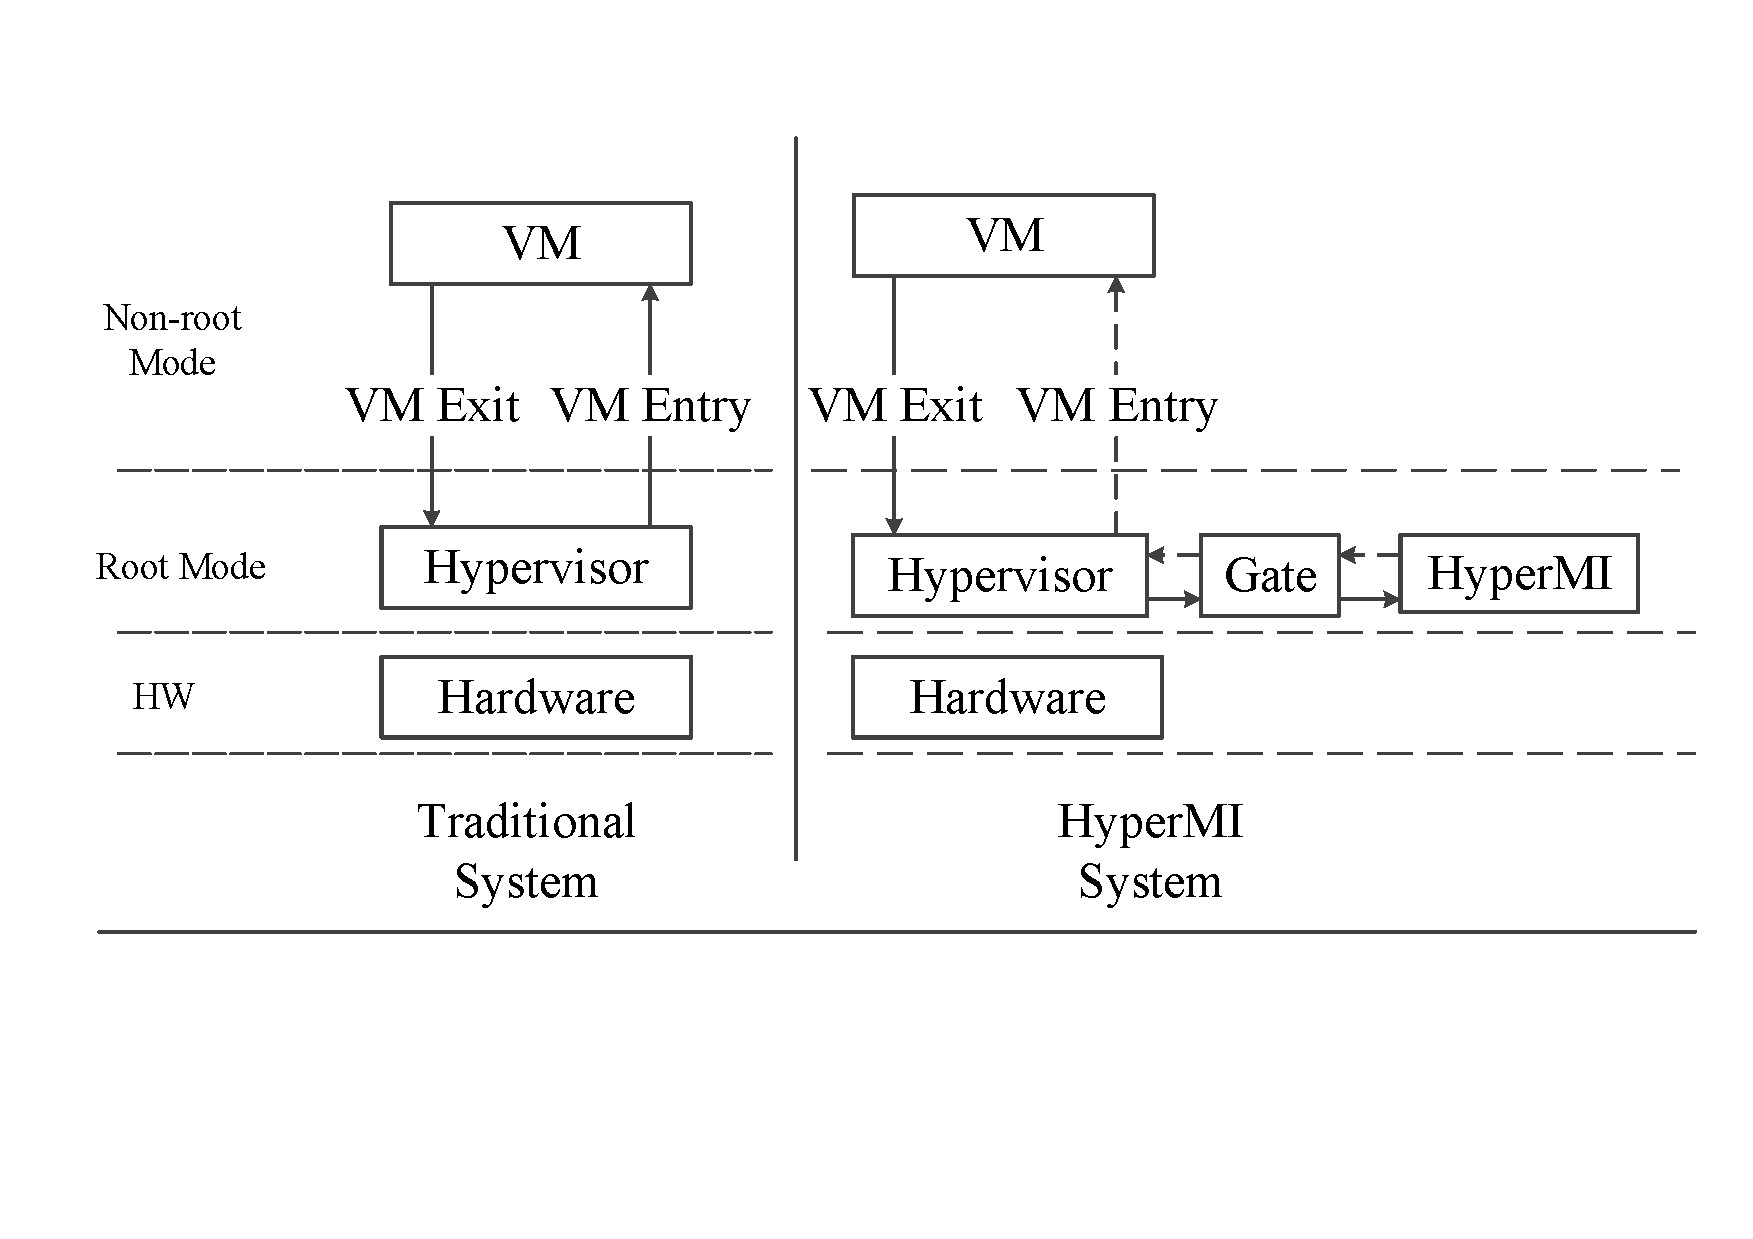
\includegraphics[width=8.5cm, height=4.5cm]{pdfvmcsProcess1-2.pdf}}%{HyprpsInteraction.pdf}}
%%\caption{Interaction comparision. } \label{fig+1}
%%\end{figure}




While the hypervisor together with guest VMs runs in Normal World, the hypervisor is forced to request HyperPS to perform two operations on its behalf: 1) switching context (VMCS monitoring) between the hypervisor and VM, 2) EPT monitoring. 
%After setting up HyperPS, the whole system is ready to create HyperPS World.
 With these designs, HyperPS intercepts and monitors VMCS and EPT access. Furthermore, HyperPS guarantees security of interaction and address translation of VMs.

%设计与实现
%架构
%交互


%
%Figure \ref{fig+1} shows the interaction process of HyperPS. 
%As described in the previous architecture, HyperPS is placed at the same privilege-level with the hypervisor, but in different address spaces. The two worlds interact through the channel, Switch Gate.
%
%
%In the original system, only guest VMs and the hypervisor are involved during the execution. In details, 1) The guest VM would deliver a trap or receive an exception to interact with the hypervisor. 2) On receiving the VM exit signal, CPU would change to root privilege from the non-root privilege. During this process, hardware would save all guest context to VMCS data structure automatically. 3) The context of the hypervisor, that is saved in VMCS too, would be loaded into registers. Then exit handler in the hypervisor gets to run. 4) The hypervisor would call VMRESUME instruction to return 6the control flow to the halted VM when exit handler is finished. The context of the guest VM stored in VMCS (the context may be modified by the hypervisor during this process) would be loaded into register. 5) The guest VM resumes to run.
%
%In HyperPS system, HyperPS hooks all functions which are involved in the interaction between the guest VM and the hypervisor. Besides, functions that are involved with EPT operation are also hooked to provide protection to EPTs. Therefore, the execution flow during VM exit has been changed on introducing HyperPS. The first two steps of VM exit are the same with that of the original system. For the third step, because the VMCS is protected by HyperPS, and the compromised hypervisor could not access this data structure. Thus, at the time, the functions used to read or write VMCS in the compromised hypervisor would be hooked and be redirected to HyperPS World, security checks would be performed to ensure the legal operation on them. It is the same with this process when functions that are involved with EPT are called. 
%After the legal operations, HyperPS would transform control flow to the compromised hypervisor to perform VMRESUME. Because VMCS and EPT is perfectly isolated and secured from the compromised hypervisor, the compromised hypervisor cannot subvert guest VMs by modifying these two most crucial data structures.






\subsection{Security-sensitive Resource Access}\label{IN}%{Interaction} \label{IN}


%Some critical data structures'(VMCS and EPT) access paths, called interaction flow, are changed based on changed stored region since these data structures are hidden in HyperPS World. 
%Figure \ref{fig+1} shows the interaction flow of HyperPS. 
For the implement, the hypervisor corresponding to Normal World should be modified to be deprived of control capabilities for security-sensitive system resources, including control registers, page table, VMCS and EPT.
In order to clarify the resource access in HyperPS World, hooks, unintended instruction elimination and interaction flow are described as follows.

\textbf{Hooks.}
We recognize control register access, page table updating, VMCS and EPT operations in Normal World as designated hypervisor events.
To tackle the threats from compromised hypervisor, hypervisor monitoring invokes the integrity assessment routines upon the occurrences of designated hypervisor events. A common approach to capture designated events is to place hooks into the origin hypervisor and eliminate related privilege instructions. These hooks can be code hooks (jump instructions) inserted at arbitrary locations in hypervisor code, or any other technique that can transfer the control flow.


\textbf{Unintended Instruction Elimination.}
Instructions composed of several fields in x86 are unintended. One or several of these fields may casually match another privileged instruction causing privilege instructions expected to be eliminated retained and hook failure. The general situation is as follows: 1)One instruction contains another privilege instruction. 2)A privilege instruction can be formed across two instructions. There is a threat that attackers jump into the middle of the instructions to execute a privileged instruction which has been eliminated and hooked by us. 
For the first case, the attack is blocked by replacing the same kind of resource, such as replacing the register in the instruction with another register. The solution to prevent the second attack is that we insert NOP instruction in the middle of these two instructions.

\textbf{Interaction Flow.}
When the hypervisor's execution reaches a hook, it will transfer the control flow to HyperPS World. By implanting hooks at the code positions where hypervisor events occur, HyperPS can capture the occurrences of designated events to assess the sensitive resource integrity.


%1 世界
%hypervisor的监控
%vmcs和ept,还有虚拟机退出
%地址隐藏还有访问函数监控,在该过程中可以拦截vmcs
%ept


%\begin{figure}
%\centerline{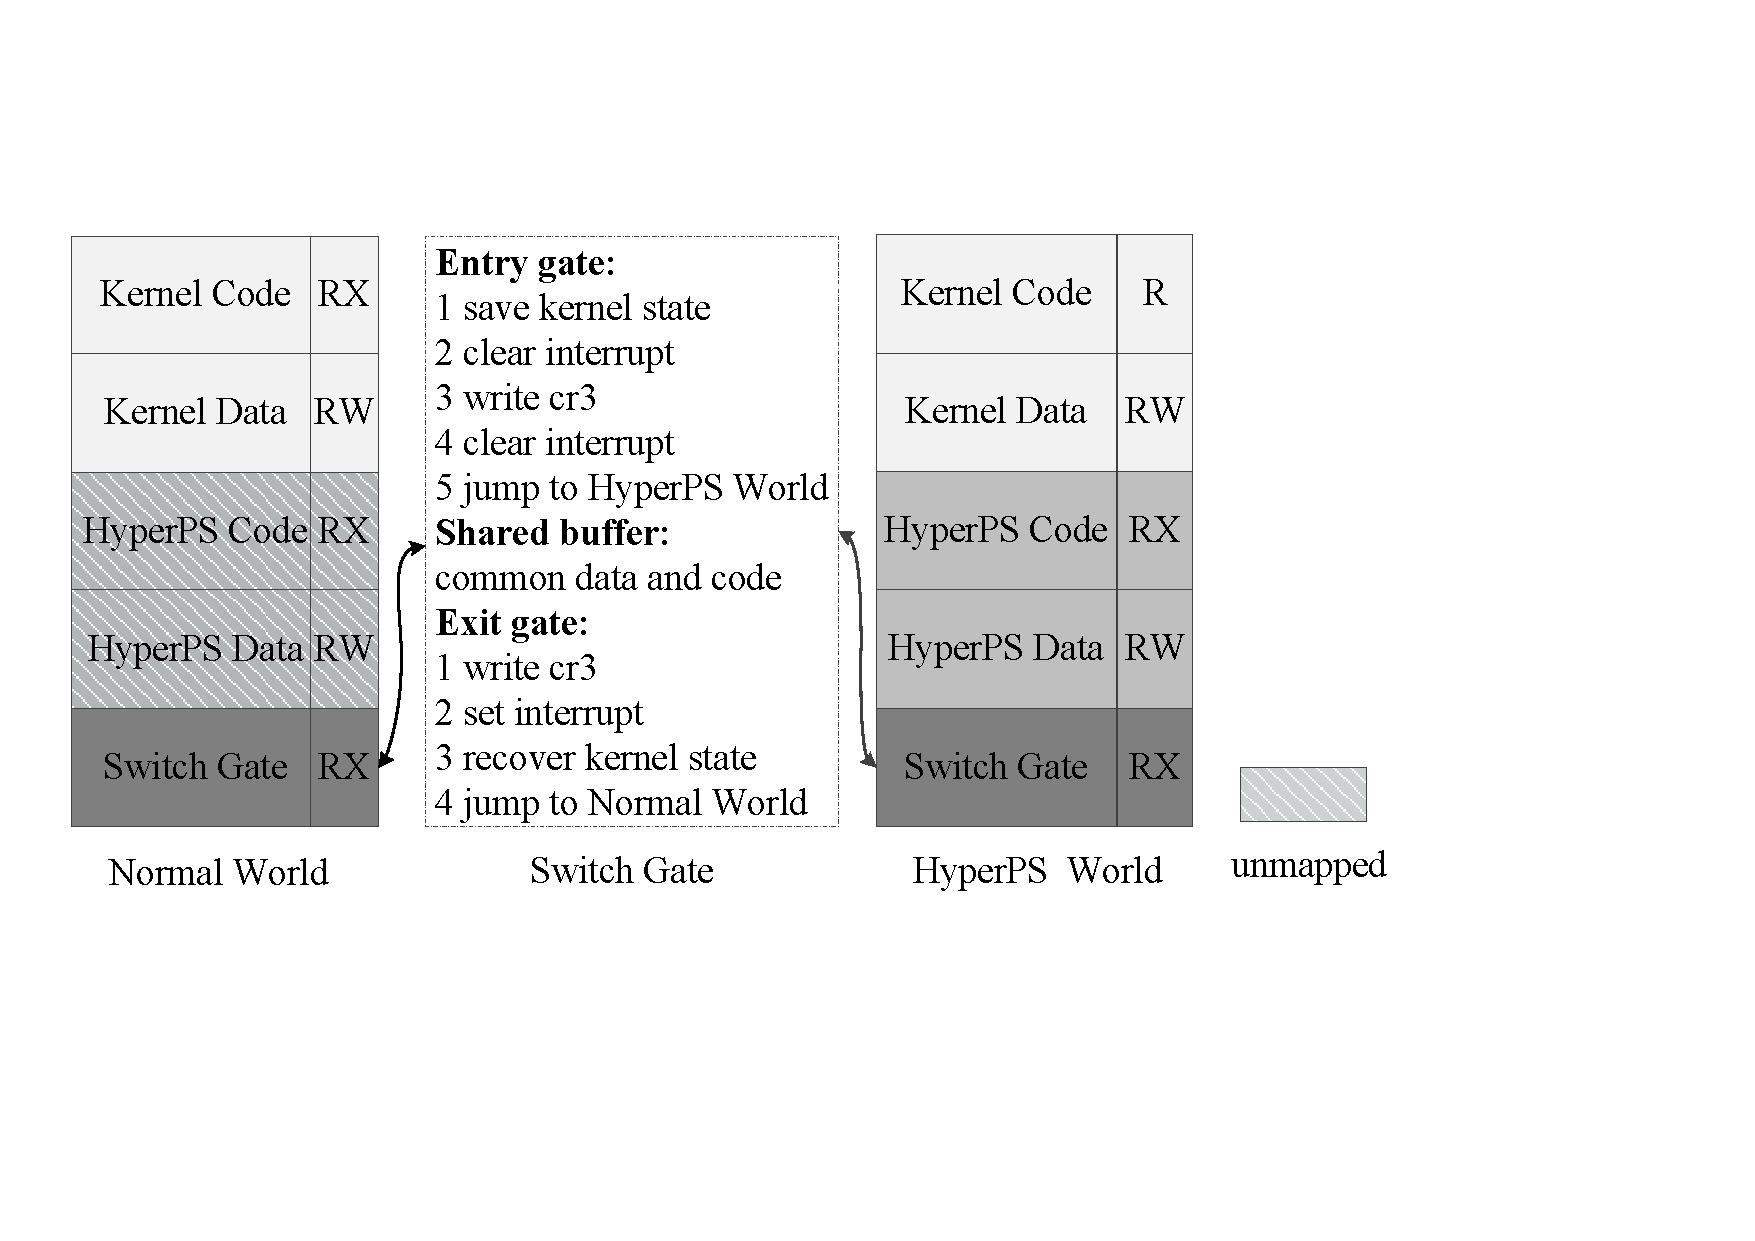
\includegraphics[width=11cm, height=7.5cm]{pdfvmcs2.pdf}}%{HyperPSLayout.pdf}}%{vmsm23.jpg}}
%\caption{An overview of address space layout.} \label{fig2}
%\end{figure}

\begin{figure}
\centerline{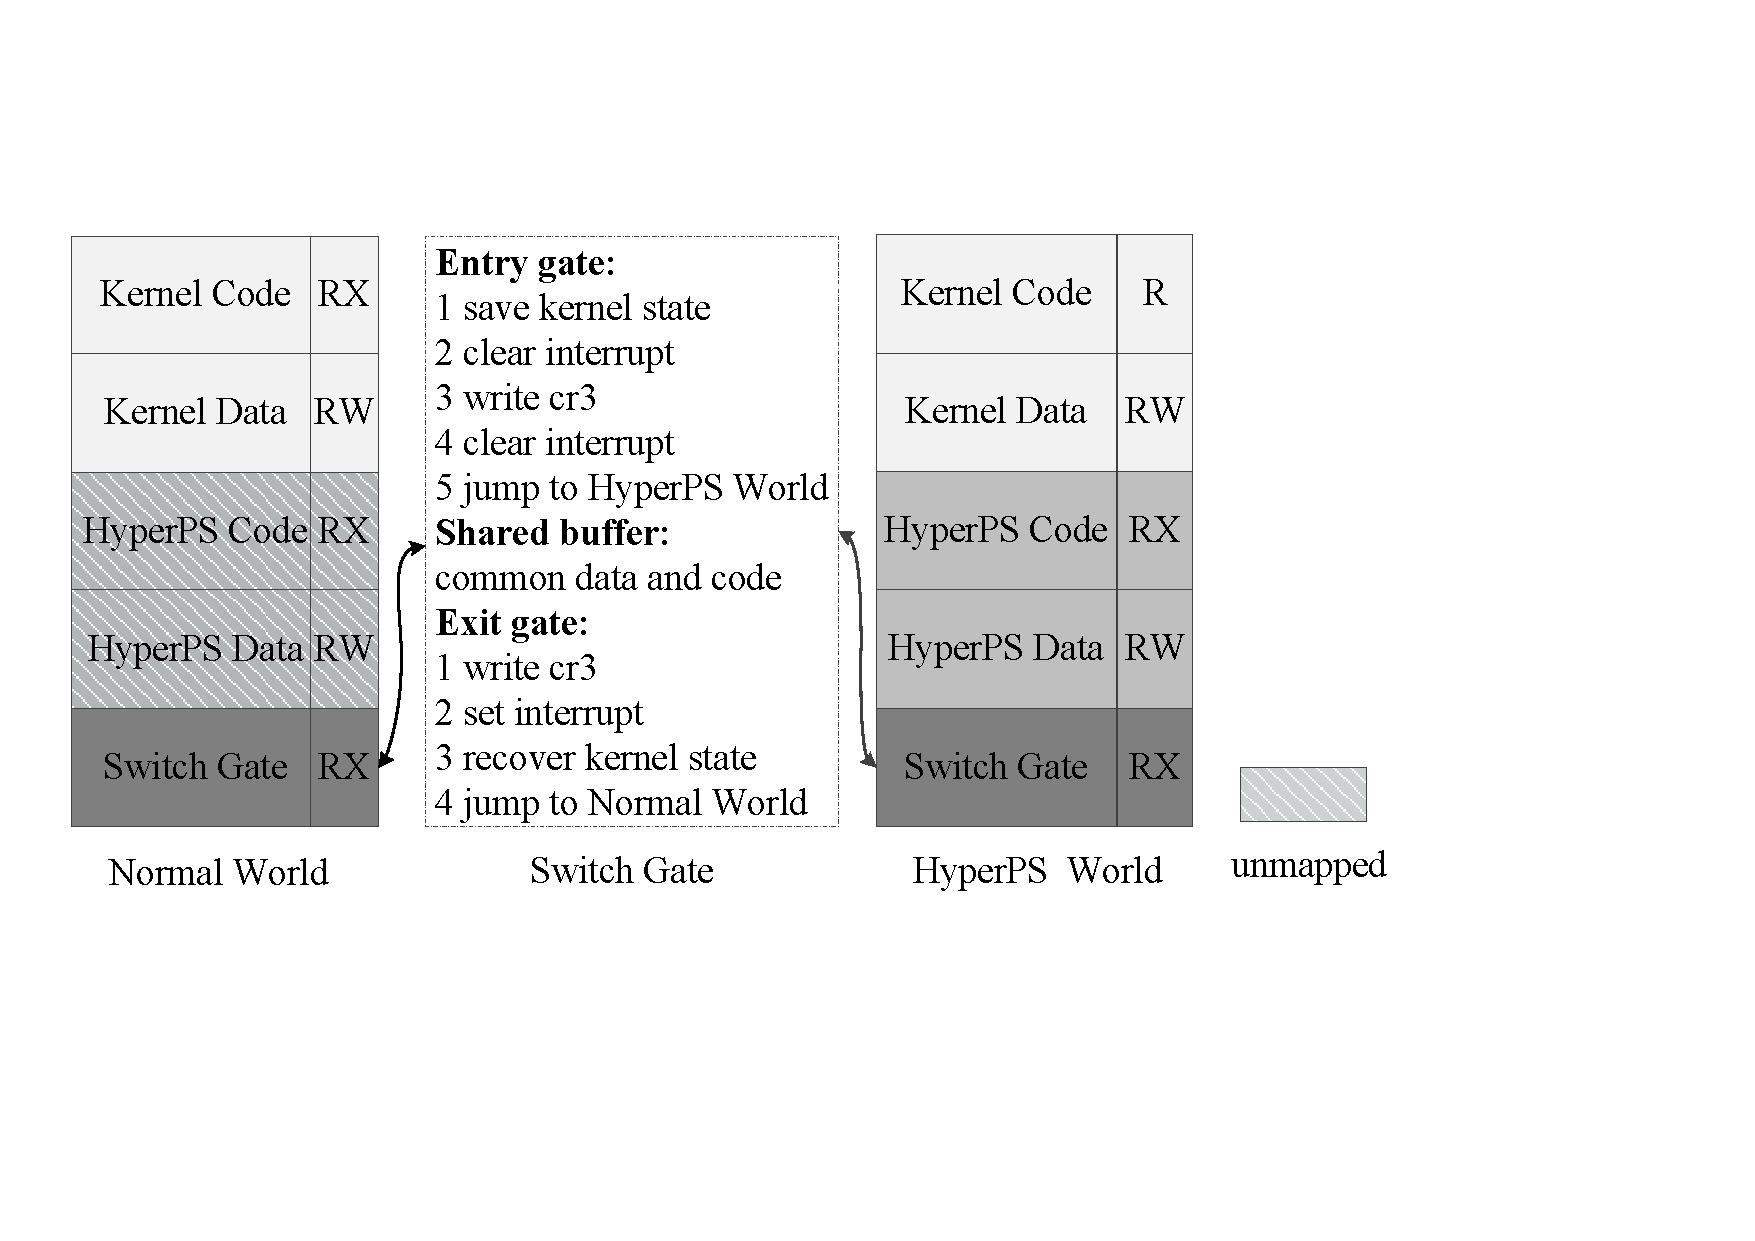
\includegraphics[width=9cm, height=5cm]{pdfvmcs2.pdf}}%{HyperPSLayout.pdf}}%{vmsm23.jpg}}
\caption{An overview of address space layout.} \label{fig2}
\end{figure}


\subsection{HyperPS World} \label {HWorld}

The creation of HyperPS World has two purposes: 1) creating a address space which can provide monitoring for VMCS and EPT. 2) creating a software system that does not depend on hardware devices and adapts to multi-system platforms. The key point of its design is that it creates address space used for privilege separation for all privilege levels at the same privilege-level with hypervisor or kernel. 
%Unlike other same privilege-level software, HyperPS World depends on another new page table and two different address spaces.

\textbf{Creating HyperPS World.}
% We use two isolated address spaces based on two sets of page tables to achieve isolation of HyperPS World.
We create another page table to achieve an isolated address space, named HyperPS World, from compromised hypervisor.
Figure \ref{fig2} describes the address space layout of two worlds through two sets of page tables, the normal page table and HyperPS page table. On the left of Figure \ref{fig2}, the normal page table contains code and data of Normal World except for that of HyperPS World. This can prevent compromised hypervisor from breaking the integrity of HyperPS World. Programs running in Normal World cannot access data in HyperPS World. On the right of Figure \ref{fig2}, all code and data segments are mapped in HyperPS page table.
HyperPS code remains executable and HyperPS data remains writable. What's the most important, kernel code is forbid to execute when HyperPS World is active, so that it cannot attack HyperPS World.






\textbf{Creating Switch Gate.}
HyperPS designs and implements Switch Gate to perform worlds switching by executing a series of ordinary instructions.
Switch Gate performs the control switching operation between Normal World and HyperPS World, acting as a wrapper function for a handler which processes incoming requests in HyperPS World. It provides Normal World with a unique way to enter HyperPS World. In addition, Switch Gate is implanted across Normal World and is invoked with specific parameters in order to handle sensitive resources including control registers, page tables, VMCS and EPT, by sending relevant requests to HyperPS World.

Figure \ref{fig2} describes the details of Switch Gate and it is divided into the entry/exit gates and shared buffer.
Entry gate provides the only entrance to HyperPS World and the exit gate provides the address for returning to Normal World. The shared buffer contains common data and code in Normal World and HyperPS World. Common code is switch code and common data includes the entry address of two sets of page tables.
% Switch Gate is mapped at the same place in Normal World and HyperPS World because switch code must be called by the two worlds before and after switching.
 Of course, the entrance address must be protected after switching to HyperPS World in case that attackers access HyperPS World causally after trusted boot. This will be introduced in section \ref{SG}.


\subsection{Hypervisor Monitoring}\label {interaction}

%\textbf{VM Monitoring}
%Our approach takes advantage of the fact that, during the runtime of a VM,
 VMCS and EPT are the most two important data structures that the hypervisor can utilize to interact with VM. %And these two data structures can only be accessed by the hypervisor in traditional virtualization environment without HyperPS. 
VMCS, the architectural in-memory structure, is used to manage the mode transitions as well as specify the restricted operations causing the VM Exit/Entry. EPT contains the mapping relationship from GPA to HPA. The VMCS can be also used to specify extended page tables (EPTs) through EPTP that control the memory access in non-root mode.
The big point of vulnerability is that the content of the VMCS and EPT would be synchronized to associated in-memory region (named VMCS region and EPT region in x86 ), the hypervisor could bypass the interception via directly accessing the region.
If the hypervisor is compromised by attackers, during the interval between VM Exit/Entry, some attacks can be conducted to subvert VM as follows. 


1) Attackers can illegally get the address of VMCS in memory region and modify the content of VMCS directly. For example, it can falsify the HOST\_RIP field causing control flow hijack attack or tampering the EPTP filed with a dedicated illegal EPT.
2) Attackers can illegally modify the content of EPT entries
%Because the EPT is responsible for managing all physical memory mapping of VM.
and conduct remapping or double mapping attack to the VM.
3) Malicious VM can load EPT of any VM and access this VM's normal memory illegally.

Obviously, the key node of attack path is to get the addresses of these two data structures.
Hence, we straightforwardly provide the protection for these data structures by using HyperPS World. These two data are hidden in HyperPS World in case of malicious access from attackers with hypervisor privilege. 
%In order to ensure that some functions can access VMCS and EPT properly, HyperPS hooks these functions into HyperPS World. 
So hypervisor requests HyperPS to handle VMCS and EPT management operations, intercept writing operations and return the corresponding result for the legal request. 

\textbf{VMCS Monitoring.}
Hardware virtualization includes a set of privilege instructions (vmptrld, vmptrst, vmclear, vmread, vmwrite) to load, store, clear, read and write the current VMCS. HyperPS intercepts the execution of these instructions by eliminating them from hypervisor's code, so that any manipulation on the VMCS can be validated by HyperPS. This is what VMCS Management in Figure \ref{fig1} does.

During VM Exit, hypervisor needs to access VM Exit reason data of VMCS, and deal with the VM exit event.
%So in case of control flow makes mistakes
Because hypervisor absents the ability to access VMCS directly, VM exit redirection is designed to finish VM Exit process. After accessing VM exit reason from VMCS in HyperPS World, the control flow switches to hypervisor and hypervisor executes VM exit event handler functions.
% VM Entry also accesses VMCS in HyperPS World. 
%The control flow is shown as Figure \ref{fig+1}.


\begin{table}[htbp]
\centering
\caption{VM-Mark Table.}\label{tab1}
%\begin{tabular}{c|c|c|c}
\begin{tabular}{p{1.4cm}|p{1.2cm}|p{1.1cm}|p{1.7cm}}
\hline
\multicolumn{4}{c}{\bfseries\textbf\centering{VM-Mark Table}}\\
\hline
{\itshape\bfseries Label} & VMID & EPTID & EPT\_Address\\
\hline
{\itshape\bfseries Description} & { The VM Identifier} & The EPT Identifier & The Entry Address of EPT\\
\hline
\end{tabular}
\end{table}


\textbf{EPT Monitoring.}
EPT plays an important role as a critical data in VM address mapping. We have stored EPT in HyperPS World to monitor all write operations on ETP so that we can block attacks on malicious writing EPT in memory region.
Some functions, EPT creating, loading, walking and destroying, need access address of EPT. It can cause system to be suspend if they cannot access the address of EPT. In order to ensure these functions can be executed normally, HyperPS places hooks on these functions, then dispatches them to HyperPS World and handles appropriately.
In the meantime, HyperPS avoids double mapping attack and remapping attack during EPT updating because of the absence of EPT in Normal World.
%, and handles remapping problems to ensure the content of page cleaned after page is swapped out. 
%This will be described in detail later.

In addition to directly accessing EPT in memory to tamper VM mapping, attackers can disrupt the isolation among EPTs by loading the EPT of another VM, indirectly access memory data on the VM.
If EPT isolation among VMs cannot be guaranteed, a malicious VM can load other VM's EPT and access the memory data. It is important to ensure EPT isolation and one VM only access own corresponding EPT.
To ensure one EPT for one VM, HyperPS creates the VM-Mark structure stored in HyperPS World as Table \ref{tab1} described. It records VMID, EPTID, EPT\_Address and binds them together. VMID is created when the VM is created. 
%and destroyed based on hash value of the image of VM.
 EPTID and EPT\_Address is recorded as long as the EPT of current VM is created. This table is destroy once the  VM is shutdown or destroyed.


\subsection{Security Guarantee for HyperPS World}\label {SG}
The security of HyperPS World guarantees the security of HyperPS, because it relies on HyperPS World to provide a trusted environment for VMCS and EPT monitoring.
Nevertheless, without any protection measures, kernel page table in Normal World is not secure for four reasons: 1) Attackers can control page table with the highest privilege after hypervisor is compromised. 2) Attackers can bypass Switch Gate to break the security of HyperPS World. 3) Attackers with the highest privilege can free to execute privilege instructions to modify the value of privilege registers, such as CR0, CR3 and so on. 4) Attackers can carry out DMA attack to access address space of HyperPS World casually.
We detail the protection measures to resist these four types of attacks below.
%\paragraph



\textbf{Protecting Page Table.}
There are three reasons for controlling the two sets of page tables: 1) To access casually or bypass HyperPS World, attackers can tamper normal page table to map address of HyperPS World or load malicious page table to CR3.
%2) To execute code injection attack, attackers can close the write protection mechanism by modifying the value of CR0 register, changing the access permission bits of the memory page. 
2) Attackers can cover the hooked functions, redirect the functions to malicious code and bypass HyperPS World.
 %interaction monitoring of HyperPS.
 3) To break HyperPS World, malicious kernel code in Normal World with execution permission can be executed to subvert HyperPS.
% by means of the vulnerabilities of the original kernel code. 
%access HyperPS World causally when HyperPS World is running if kernel code has the execution permission. 
%Therefore, three secure approaches against these attacks are as follow.

For the first attack, %HyperPS code and data is unmapped in page table of Normal World.
% And to protect the entrance address to HyperPS World from being leaked,
%pre-allocate some space during trusted boot which kernel can't access directly through MMU, critical data in
we remove all entries that map to HyperPS World from the page table in Normal World and deprive the ability to access CR3 of the kernel. % in order to avoid loading illegal page table, and resist bypassing HyperPS World.
For the second attack, we intercept the accessing operation to CR0 and maintain the WP bit as 1. We stick to W$\oplus${X} and maintain the code segment of hooked functions unwritable.
For the third attack, we set the kernel code segment as NX (non-executable) when HyperPS World is running. For more security, we modify the kernel to configure these two sets of page table as read-only by setting the page tables page unwritable. This is necessary to prevent the page tables from being modified by attackers. Privilege instructions about page fault and setting pte are hooked and trapped to HyperPS World. Any write permission modification of two sets of page table must cause the kernel to page fault, then we dispatch page fault to HyperPS World to verify the correctness of address mapping. 
%This idea is adopted in SKEE\cite{Azab2016SKEE}.


\textbf{Worlds Switching Securely.}
HyperPS creates Switch Gate between Normal World and HyperPS World by loading entry address of page table into CR3.
In order to ensure switch security, we design the switch process as follows.
% And we must ensure atomicity and security during the switching process.

The switching process described in Figure \ref{fig2} is as follows: 1) Save the kernel state to the stack including general registers and interrupt enable/disable status. 2) Clear the interrupt with the CLI instruction. 3) Load the page table to the register CR3. 4) Interrupt again. 5) Jump to the HyperPS World. For the exit process, the control flow returns to Normal World by performing the operations in the reverse order.


\textbf{Accessing Control Registers Securely.}
The hypervisor without HyperPS is privileged and it can free to execute privilege instructions, so that it can write any value to the related control registers. 1) Malicious attackers can close DEP mechanism by modifying CR0, close SMEP mechanism by modifying CR4. 2) Kernel code can load a crafted page table to bypass HyperPS World by converting a meticulously constructed address of one page table to CR3.
To prevent these, HyperPS deprives sensitive privilege instructions executed by the hypervisor, and dispatches captured events to HyperPS World. HyperPS World can choose how to handle this event, such as executing, issuing alerts or terminating the process. 

\textbf{Resisting DMA Attack.}
%Thirdly, it is important to focus on DMA attack. 
DMA operation is used by hardware devices to access physical address directly. Malicious attackers can read or write arbitrary memory regions including HyperPS World by DMA. Therefore, it is a crucial focus of intercepting direct access to physical pages belonging to HyperPS World by DMA operation. 
Fortunately, HyperPS employs IOMMU mechanism to avoid DMA attack, which can carry out access control for DMA access. Our approach adopts two policies: 1) We remove the corresponding mapping of the critical data from the page table which IOMMU uses. These critical unmapped data includes the entrance address of HyperPS, data recording VM-Mark structure used in EPT management and so on. 2) HyperPS intercepts the address mapping functions about I/O, verifies whether the address belongs to the address space of HyperPS World, then chooses to map or unmap.


Through the above security measures, HyperPS can be protected from being bypassed and being broken, thus providing a secure execution environment for hypervisor monitoring.




%对域的保护

%实现
%
%创建世界 门 启动 
%
%安全分析
%自身的安全分析
%对交互数据和EPT的安全分析

%
%评估
%1 安全
%照写
%
%2 性能测试
%总体的beachmark 
%lmbeach
%空的切换
%虚拟机的启动关闭时间


%当前的系统往往是一体化的,为了达到一定的权限分离,原先的一些基于x86处理器的研究提出了基于WP保护的方案。这些方案通过对指向内部域的页表实现写保护来保护是内核,并没有连同保护hypervisor。The greatest strength of these researches on privilege separation is that it can provide the same write protection for virtually all privilege levels and types of system software on the x86 processor. 
%后期的一些研究提出了对
%some researchers diversify their intra-level privilege separation solutions for different levels of privileged software on x86 machines like those for an OS [15] and for a hypervisor [46].
%In modern software architectures, it is by no means unusual for more than one levels of system software to coexist in a system. The most familiar case found in a real system would be that an OS is installed together with a hypervisor. 



\section{Evaluation}\label{sec:evaluation}
%We describe the design and implementation of HyperPS. 
%In this section, we evaluate the protection effectiveness and performance of HyperPS by exploiting vulnerabilities and comparing it with traditional KVM through a set of benchmarks.
In this section, we first analyze the security guarantees provided by HyperPS. Then, we evaluate the performance overhead by running a set of benchmarks on both standard KVM and HyperPS.



\subsection{Security Analysis}
 
%In section \ref{sec:design}, we discuss in detail how HyperPS achieves memory isolation, and secure interactions between VM and the hypervisor. Just as the threat model described in the section \ref{threat}, an attacker could subvert the upper VMs by conducting attacks such as cross-domain attack with a malicious virtual machine.
In this section, we elaborate the security evaluation on how HyperPS achieves hypervisor monitoring through monitoring VMCS and EPT manipulations. 
In addition, we analyze the security of HyperPS itself. Table \ref{tab3} shows the real attack instances in line with the above attack model. 

%However, these two attack vectors, regardless of their attack path, both focus on critical interaction data and data on memory, afterwards, modifying more detailed data, such as the VMCS data structure, EPT and EPT Pointer. Thus, we will elaborate on how HyperPS fends of these attack, and Table \ref{tab3} shows the two real attack instances in line with the above attack model. 
% the attack instances listed in Table \ref{tab3} perfectly match the description of attacker, so we will use these two instances to specifically analyze security performance. 


\textbf{Modifying VMCS Attack.}
We clarify the importance of protecting interaction data including VMCS in Section \ref{interaction}.
% To prevent interaction-data leakage, we protect VMCS from attackers.
 Firstly, VMCS is hidden in HyperPS World and cannot be accessed by hypervisor. Secondly, functions that can access VMCS are hooked into HyperPS World, therefore, no functions outside HyperPS World can access VMCS. Attackers cannot get location of VMCS and access it. This prevents attackers from tampering interaction data. We examine protection for VMCS by conducting several attack cases which are widely adopted in real world. 
%Table \ref{tab3} lists all attack cases we used. The modifying VMCS attack, tries to tamper the Guest\_CR3 field in VMCS. This attack fails because it cannot access VMCS. 
% The experimental results show that the access failed, malicious interaction-data accessing is prevented successfully.
 % According to the above analysis, attackers cannot access VMCS, and cannot conduct further attacks. 
The modifying VMCS attack, one of attack cases listed in Table \ref{tab3}, which tries to tamper the Guest\_CR3 field of VMCS, fails because it loses the access privilege to VMCS. According to the above analysis, attackers cannot conduct further attacks which rely on VMCS access.


%CVE-2009-2287 allows attacker to provide invalid value of CR3, which is an important data value in VMCS data structure. Because HyperPS would check the value of CR3 before VM entry instruction is conducted, an attacker has no chance to load the value to physical CR3 register successfully. HyperPS protects all important data values in VMCS data structure. In details, interaction between hypervisor and VMs runs in HyperPS World, VMCS structure used to record context switching data is hidden in HyperPS World, so an attacker cannot modify VM states during context switching. HyperPS adopts VM-Mark table to ensure that load consistent EPT for every VM, so attacker cannot modify EPTP. Therefore, the VM states cannot be modified. 




\textbf{Subverting Memory Across VMs Attack.}
%A kind of attack is subverting memory protection across VMs. 
%Original hypervisor manages the memory of VM through EPT which controls the address translation of VM, so compromised hypervisor can incur malicious memory access attack, such as double mapping attack and remapping attack. However, HyperPS hides the address of EPT in HyperPS World and hooks all operations about EPT into HyperPS World. Page tracking technology can make and prevents double mapping and remapping attack. Page tracking technology can ensure that each physical page has only one owner, verify the ownership of each physical page when EPT updates the mapping, and ensure the safe mapping of physical memory. Page tracking  technology can clear the contents of pages when they are completely released, ensuring information security.
%
The main attacks that attackers can execute on subverting memory are double mapping attack and remapping attack by modifying EPT entry.
Firstly, double mapping attack succeeds by allocating memory pages that have already been owned by a hostile VM to a victim VM. Secondly, another challenge is page remapping attack by a compromised hypervisor from a victim VM to a conspiratorial VM. This attack involves remapping a private page to another virtual address.
The absence of EPT in Normal World can prevent modification from attackers because they cannot access EPT in memory region directly.

%Page marking and write-protection of EPT prevent this kind of attack. For each new mapping to a VM, HyperPS validates whether the page is already in use according to Used field of Page-Mark structure. Meanwhile, the allocated pages must be marked in the Page-Mark table for tracking. Secondly, another challenge is page remapping attack by a compromised hypervisor from a victim VM to a conspiratorial VM. This attack involves remapping a private page to another virtual address. To defeat this type of attack, HyperPS ensures that whenever a page is released, its content must be zeroed out before creating a new mapping.


We implement a real attack by exploiting CVE-2017-8106 in kernel version 3.12. A privileged KVM guest OS user accesses EPT, conducts attacks via a single-context INVEPT instruction with a NULL EPT Pointer. Attackers cannot implement successfully and incur EPT access fault because HyperPS hides the address of EPT in HyperPS World and hijacks the loading of EPT. HyperPS verifies the value of EPT to avoid loading NULL value. Therefore, HyperPS can avoid subverting memory across VMs including double mapping attack, remapping attack as well as malicious EPT access.
% attacker is unable to subvert the upper VMs by exploiting the hypervisor vulnerability. 
%But an attack on memory is not limited to loading malicious EPT Pointer.


\begin{table}
\centering
\caption{Hypervisor Attacks Against HyperPS.}\label{tab3}
\begin{tabular}{p{2.8cm}|p{5.5cm}}
\hline
{\itshape\bfseries Attack} & {\itshape\bfseries Description} \\
\hline
Modifying VMCS Attack & Load a crafted GUEST\_CR3 value\\
\hline
CVE-2017-8106 & Load a crafted EPT value \\
\hline
DMA Attack & Access HyperPS World by DMA \\
\hline
Code Injection Attack & Inject code and cover hooked functions to bypass HyperPS World \\
\hline
\end{tabular}
\end{table}

\textbf{Destroying HyperPS World.}
HyperPS World is created by relying on new page table.
% When HyperPS does not work, the original kernel with high privileges can access any page tables and modify them. It can also access control registers casually, redirect hooked functions used to monitor previously, and even maliciously destroy HyperPS World through DMA. 
We analyze the protection for HyperPS World from four aspects, page table modification attack, hooks redirection attack, register modification attack and DMA attack.


\subsubsection{Page Table Modification Attack}

Page table protection has been introduced in section \ref{SG}. The entry address mapping of the HyperPS page table is deleted from the old page table to prevent the kernel from accessing HyperPS World directly through the page table mapping. 
%When HyperPS World is active, the kernel code does not have any executable permissions in case of attacking running processes in HyperPS World. 
When HyperPS World is active, the kernel code does not have any executable permissions to prevent attacking a  process running in HyperPS world.
Attackers may attack in two ways.
First, attackers may try to directly access the new page table address on the kernel page table by virtual address mapping. When he accesses it, there is page fault due to the absence of virtual to physical address mapping.
Second, attackers may run kernel code while HyperPS World is active to attack programs running in HyperPS World. This can be prevented because of the absence of executable privilege of kernel code.



\subsubsection{Hooks Redirection Attack}

Due to the code of hooked functions including page table updating, control register access operations and VMCS operations, EPT operations, are writable-protection. Accessing CR0 register operation used to set W$\oplus${X} is controlled and page table updating used to change code execution privilege is limited, attackers cannot redirect hooked functions and bypass monitoring.

\subsubsection{Register Modification Attack}

Some register access operations including CR0, CR3, CR4, are controlled and hooked to HyperPS World. 
HyperPS completes the update and monitoring of registers to ensure that the security mechanism is enabled while the system is running. 
%CR0 register can control the W$\oplus${X} privilege of code, CR3 can control the loading of the page table and CR4 can decide SMEP mechanism.
 Protection for page table, hooked functions and registers, plays a role mutually in protection for HyperPS. 

\subsubsection{DMA Attack}

%In addition, the memory can be accessed through DMA operations bypassing the MMU, except for accesses by executing memory accessing instructions.
 DMA attack is described in detail in section \ref{SG}. Attackers can use this feature to read or corrupt arbitrary memory regions. DMA attack is not a threat to HyperPS, because HyperPS is inherently secure against DMA using IOMMU. We remove the corresponding mapping of the critical data from the page table which IOMMU uses. These critical unmapped data includes the entrance address of HyperPS, VMCS, EPT and VM-Mark structure. 
HyperPS intercepts the related functions of the DMA mapping and verifies that the physical address to be mapped is not within the scope of the critical data address during the DMA mapping process.
DMA attack that aims at modifying the VM memory or the page tables can also be defeated.

%\begin{figure}
%\centerline{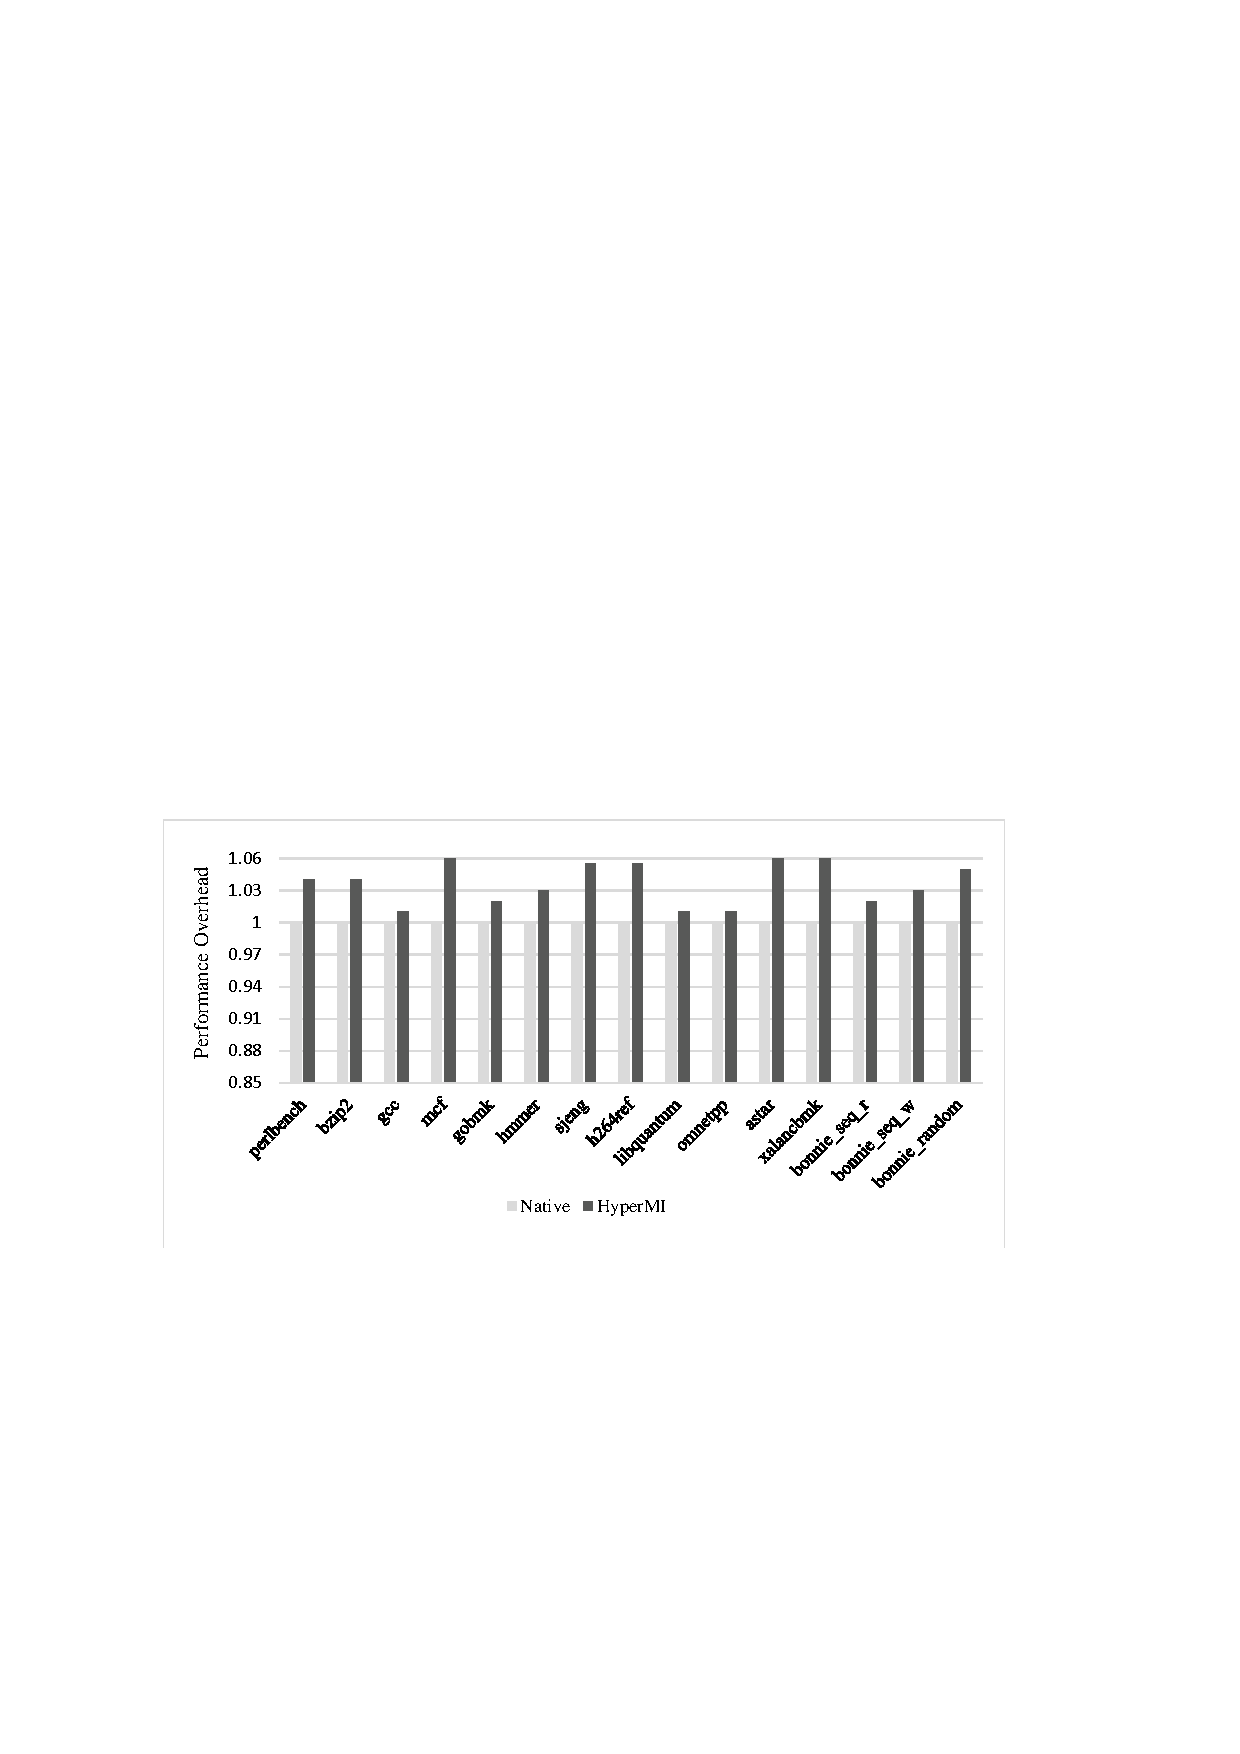
\includegraphics[width=9cm,height=5.2cm]{performance.pdf}}
%\caption{Performance overhead.} \label{fig5}
%\end{figure}

\begin{figure}
\centerline{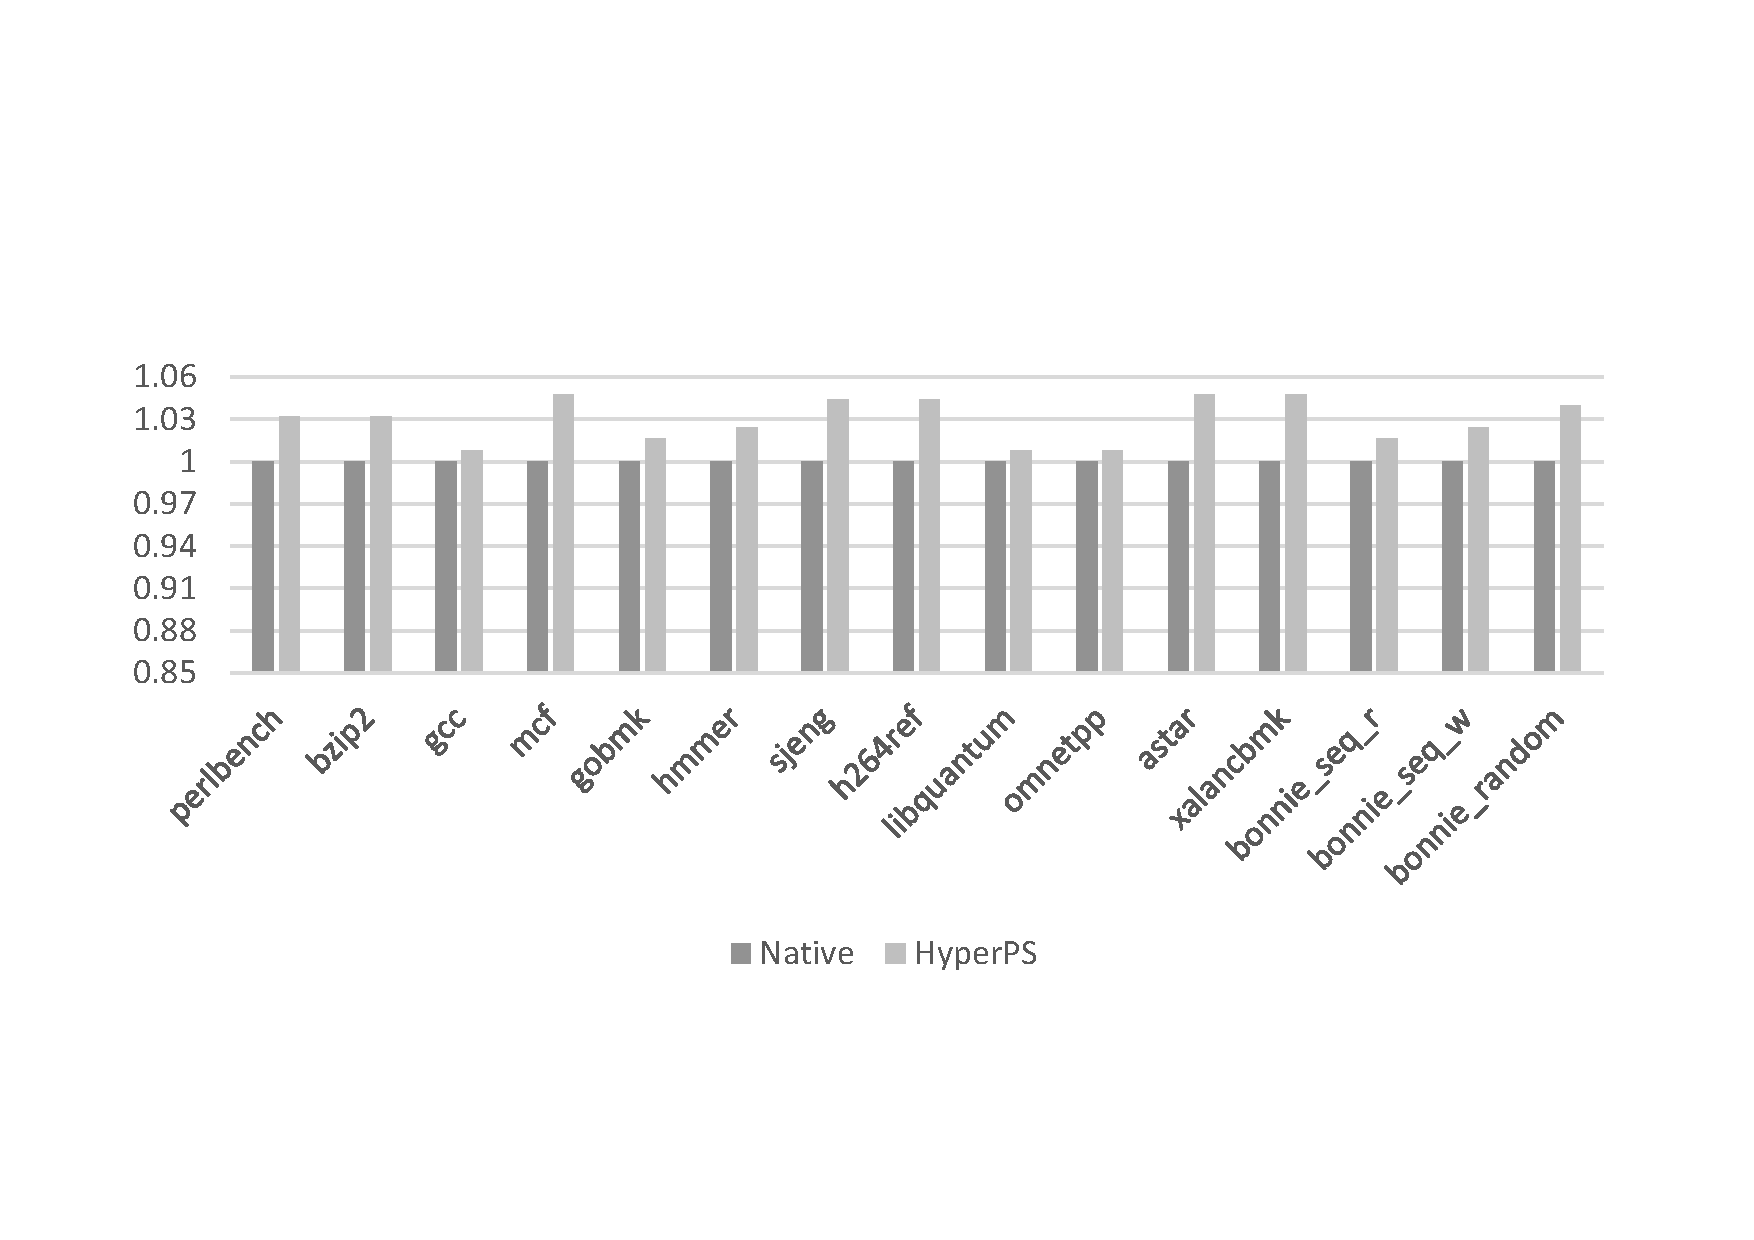
\includegraphics[width=8cm,height=4.3cm]{performance2.pdf}}
\caption{Performance evaluation.} \label{fig5}
\end{figure}


\subsection{Performance Evaluation}

In HyperPS, the hypervisor is modified so that HyperPS World is initialized during the boot up sequence. This includes creating a new memory page table for HyperPS, allocating memory pages. VM startup can cause memory allocation and I/O access. 
%VMCS and EPT access as well as VM Exit/VM_Entry. 
These processes introduce security accessing and verification for VMCS in HyperPS World during VM Exit/Entry sequence.
The hypervisor is modified to place hooks upon some sensitive system resources, including control registers, page table, VMCS and EPT,
%control registers, accessing VMCS operations, and accessing EPT operations。
% in order to achieve HyperPS World, VM Monitoring and VM Isolation.
% The contorl flow jumps to HyperPS World through Switch Gate. 
introducing worlds switching overhead using Switch Gate.

%We do not directly compare HyperPS with previous software approaches, as they cannot support all functions simultaneously. 
In order to assess the effectiveness of all aspects of HyperPS, we conduct a set of experiments to evaluate the performance impact imposed by HyperPS against an original KVM system (the baseline). We run two groups of experiments, compare the performance overhead including benchmarks performance overhead and VM load time.
%. 
For simplicity, we only present the performance evaluation on a server with 64 cores and 32 GB memory, running at 2.0 GHz and guest VM with 2 virtual cores. The version of the hypervisor and guest VM is 3.10.1. Different experiments are based on different numbers of guest VMs with different memory size. Both the original hypervisor and HyperPS systems have the same configuration except the protection supported by HyperPS. The deviation of these experiments is insignificant. All the experiments are replicated fifty times and the average results are reported here.



\textbf{Benchmarks Performance.}
%All experiments are done on a server with 64 cores and 32 GB memory, running at 2.0 GHz and 5 VMs. 
In order to obtain the impact of HyperPS on the whole system, we measure HyperPS with microbenchmarks and application benchmarks. 
We use one guest VM with 1 GB memory size. 
%All experiments are done 50 times and results are from the average.

To better understand the factor causing the performance overhead, we experiment with compute-bound benchmark (SPEC CPU2006 suite) and one I/O-bound benchmark (Bonnie++) running upon original KVM and HyperPS in a Linux VM. The experiment result described in Figure \ref{fig5} (the last three groups) shows a relatively low cost. Most of the SPEC CPU2006 benchmarks (the first twelve groups) show less than 4.8\% performance overhead. It's not surprising as there are few OS interactions and these tests are compute-bound. Mcf, astar, and xalancbmk with the highest performance loss allocate lots of memory. HyperPS verifies the legality of EPT when EPT updates. This can incur worlds switching which involves controlling register access and incur VM Exit which involves EPT updating.
% and fewer TLB flushes with PCID technique because the two worlds are at the same privileged layer.
 For Bonnie++, we choose a 1000 MB file to perform the sequential read, write and random access. The performance loss of sequential read, write and random access is 1.6\%, 2.4\% and 4\%, not high, the main reason is that HyperPS has no extra memory operations for I/O data. The performance result shows that HyperPS introduces trivial switch overhead of two worlds and trivial overhead of monitoring hypervisor.

%{\bfseries\textbf\centering{Page-Mark Table}}
\begin{table}
\centering
\caption{execution time of vm operation(s).}\label{tabvm}
%\begin{tabular}{|c{1cm}|c|c|}
\begin{tabular}{p{2cm}|p{1.4cm}|p{1.5cm}}
\hline
{\itshape\bfseries  Test Case} & {\itshape\bfseries VM Create} & {\itshape\bfseries VM Destroy} \\
\hline
No\_HyperPS & 10.54 s &  2.34 s\\
\hline
With\_HyperPS & 11.49 s & 2.50 s\\ 
\hline
Efficiency & 1.09 & 1.07 \\
\hline
\end{tabular}
\end{table}


\textbf {VM Loading.}
% and World Switch Overhead}
VM load time is a critical aspect of performance to be considered because it influences user experience.
% We design experiments to evaluate the performance impact of HyperPS for VM loading.
 Experiments are done with 3 VMs, each guest VM is with different memory sizes from 512MB to 2GB.
 As expected, the VM booting time in HyperPS increases as the memory sizes increase, and the growth amplitude is larger due to the worlds switch and VMCS, EPT access.
%and page tracking caused by frequent memory allocation.
In addition, we measure the impact of completely booting and shutting down a VM (configured with 2 VCPU and 512MB memory). As Table \ref{tabvm} shown, the booting time is suffered a 1.09 times slowdown under HyperPS, shutdown time is suffered a 1.07 times slowdown, due to the extra overhead of worlds switching and VM-Mark table accessing in HyperPS World. %Such overhead is worth for HyperPS.


\iffalse
\textbf {VM Exit/Entry Overhead}
Experiments are done on one VM with 2G memory. Network accessing can introduce lots of VM Exit, afterwards VMCS accessing in HyperPS World and world switches. In order to measure the performance impact of HyperPS, we use Netperf (version 2.7.0), a benchmark for measuring various aspects of networking performance, to determine VM Exit/Entry performance overhead. We run a netperf process in the tested VM, sending TCP or UDP streams. The performance of I/O instruction exits (i.e., VM exits triggered by the guest's I/O requests) is 2\% for TCP and 3\% for UDP, not high. 
%When we send or receive 1024-byte packets to or from an external server, HyperPS introduces xxx times VM Exit per second, xxx\% less than original KVM. 
Based on experimental results, we conclude that VMCS accessing in HyperPS World and worlds switching can be accepted.

\fi

\section{Related work}\label{sec:related}
We describe the related work from these three aspects,
% integrity verification for hypervisor,
privilege separation, TCB reduction, and the same privilege-level isolation.
% The first aspect is considered from the perspective of protecting the hypervisor, and the other three aspects are considered from the perspective of protecting VMs.

%\subsection{Protection for Hypervisor}
\iffalse

\subsection{Integrity Verification for Hypervisor}
In order to ensure the security of the hypervisor during trusted boot and runtime, an effective and commonly used method is to verify the integrity of the hypervisor, and reduce the attack surface. For the security of the hypervisor during trusted boot, paper \cite{Petroni2007Automated} proposes control flow integrity protection policy, by verifying regularly control flow integrity behavior to detect rootkit attacks. However, attacker can detect the regular and bypass the detection. For runtime security of the hypervisor, HyperSafe \cite{Wang2010HyperSafe} and HyperCheck \cite{Wang2010HyperCheck} choose pooling-query method based on SMM to finish integrity verification of hypervisor. However, SMM doesn't support for MMU. And attackers can hide trace during polling-query intervals when comparing to event-driven monitoring.
\fi


%\subsection{Resource Isolation}

%\subsection{Customized Hardware }
%Some works at hardware level complete the protection of the process by extending the virtualization capabilities\cite{Moon2012Vigilare},\cite{Lee2013KI}. These tasks provide fine-grained isolation of processes and modules from the hardware level. Haven \cite{haven} uses Intel SGX\cite{Hoekstra13cuvillo,Mckeen2013Innovative} to isolate cloud services from other services and prevent cross-domain access. SGX provides fine-grained protection at the application space instead of hypervisor space, and needs developers spend time reconstructing code and dividing code into trusted part or untrusted part. SGX has requirement for version of CPU and is applied on a few platforms.
%
%The effort \cite{Cho2016Hardware} combines the advantages of ARM TrustZone and virtualization to improve system performance, and isolate critical process components securely and efficiently.
% H-SVM\cite{Jin2015H} utilizes the hardware extension features of the CPU, and extends SMM microcode to achieve memory resource isolation among virtual machines. It deprives ability of accessing to memory resource by replacing the source code of the original hypervisor to access memory resource.
% Vigilare\cite{Moon2012Vigilare} and KI-Mon \cite{Lee2013KI} provide monitoring for access operations by introducing extra hardware. Vigilare provides a kernel integrity monitor that is architected to snoop the bus traffic of the host system from a separate independent hardware. 
% It adds extra Snooper hardware connections module to the host system for bus snooping. KI-Mon monitors write operation to system bus and handles data to write in order to check rootkit attack.
%However, for cloud providers, these approaches means high-cost and low practicality as long as they are carried out widely.
%KI-Mon monitors write operation on system bus and handles data to write in order to check rootkit attack.

%\subsection{Reconstructed Hypervisor }
%Except for approaches based on hardware, some works\cite{nexen,Steinberg2010NOVA,hyperlock} pay attention to software isolation. Pre-allocating physical resource and completed isolated environment for every VM can avoid VM cross-domain attack, and data leakage attack. NOVA\cite{Steinberg2010NOVA} divides hypervisor into micro-hypervisor and user hypervisor running in root mode, adopts an idea which is similar to fault domain isolation to guarantee an isolated user hypervisor for every VM. 
%The drawback of this approach is the lack of fractional traditional hypervisor functions.
% HyperLock \cite{hyperlock} prepares backup KVM for every VM by copying KVM code, and ensures every VM run in own isolated space. 
%Nexen\cite{nexen} reconstructs the XEN hypervisor into one privileged security monitor, one component for shared service, backup XEN code and data for every VM, to resist attacker from exploiting known XEN vulnerabilities. 
%These approaches redesign hypervisor greatly. In contrary, HyperPS adopts a feasible way to isolate VM without lots of modification of hypervisor. 

\subsection{Privilege Separation}
Some works\cite{nexen,Steinberg2010NOVA,hyperlock,dehy} pay attention to privilege separation. Pre-allocating physical resource and providing privilege separation for every VM can avoid VM cross-domain attack, and data leakage attack. Some efforts\cite{Moon2012Vigilare} and KI-Mon \cite{Lee2013KI} provide monitoring for access operations to critical data by introducing extra hardware.
%DeHype\cite{dehy} further demotes the KVM module to user mode and applies the least privilege
principle to it.
 NOVA\cite{Steinberg2010NOVA} divides hypervisor into microhypervisor and user hypervisor running in root mode, adopts an idea which is similar to fault domain isolation to guarantee privilege separation for every VM. Some of them redesign hypervisor greatly. In contrary, HyperPS adopts a feasible way to separate privilege without lots of modification of hypervisor. 

%\subsection{Hypervisor Monitoring}
%In order to ensure the security of the hypervisor during trusted boot and runtime, an effective and commonly used method is to monitor
%%verify the integrity of 
%the hypervisor, and reduce the attack surface. For the security of the hypervisor during trusted boot, paper \cite{Petroni2007Automated} proposes control flow integrity protection policy, by verifying regularly control flow integrity behavior to detect rootkit attacks. However, attacker can detect the regular and bypass the detection. For runtime security of the hypervisor, HyperSafe \cite{Wang2010HyperSafe} and HyperCheck \cite{Wang2010HyperCheck} choose pooling-query method based on SMM to finish integrity verification of hypervisor. And attackers can hide trace during polling-query intervals when comparing to event-driven monitoring.

\subsection{TCB Reduction}
Reducing TCB can reduce the possibility of the whole system being attacked by reducing the amount of hypervisor code, changing the organizational structure of virtualization, even reducing the interaction between VM and hypervisor.
HyperLock\cite{hyperlock} removes the KVM module from the TCB using the combination of address space isolation and software-based fault isolation (SFI). DeHype\cite{dehy} further demotes the KVM module to user mode and applies the least privilege. Mycloud\cite{mycloud} and MycloudSEP\cite{Detangling}, on the other hand, deprivilege the execution of the host VM in non-root mode and remove it from TCB.


\subsection{The Same Privilege Level Isolation}
Some efforts, 
%ED-Monitor\cite{Deng2017Dancing},
\cite{Azab2016SKEE},\cite{Wang2015SecPod},\cite{Deng2017Dancing}, adopt the same privilege-level idea to achieve privilege separation and avoid performance overhead of inter-level translation.
%///////////////////
% ED-Monitor presents a novel approach that enables practical event-driven monitoring for compromised hypervisor in cloud computing, adopts "the same privilege level" protection against an untrusted hypervisor. The created monitor is placed at the same privilege level and in the same space with hypervisor. It relies on the mutual-protection of an
%unique pair of the techniques: Instrumentation-based Privilege Restriction (IPR) and Address Space Randomization (ASR). At the high level, IPR intercepts the most privileged operations in the Hypervisor and transfers these operations to ED-monitor, while ASR hides ED-monitor in the address space from the Hypervisor.
% SKEE provides a lightweight secure kernel-level execution environment, it is placed at the same privilege-level with kernel. SKEE is exclusively designed for commodity ARM platforms using system characteristics of ARM. 
%///////////////////
% can only be applied to limited levels of system software in comparison with HyperPS.
SKEE\cite{Azab2016SKEE} is one of the most notable work to realize privilege separation on ARM's commodity processors today. 
However, SKEE is not commonly applicable to different levels of system software in comparison with HyperPS, such as hypervisors because it is designed for different hardware feature which is only defined in the kernel privilege level on ARM's 32-bit or 64-bit architecture.
%///////////////////
%SKEE is more focused on using the features of the ARM platform while HyperPS has no dependence on multi-platforms. 
% First, targeting ARM's 32-bit architecture, SKEE capitalizes mainly on Translation Table Base Control Register (TTBCR) for dynamic page table activation. To be more specific, SKEE creates separate page tables for the secure world and activates it in a timely manner by modifying the N field of TTBCR. However, as this hardware feature is only defined in the kernel privilege level on AArch32, SKEE is not commonly applicable to different levels of system software, such as hypervisors.
% Unfortunately, SKEE faces a similar limitation on ARM's 64-bit architecture. SKEE is more focused on using the features of the ARM platform while HyperPS has no dependence on multi-platforms.
%The difference between HyperPS and SKEE is that HyperPS uses two sets of page tables to create the execution environment, and SKEE uses one set of page table. The design of Switch Gate for HyperPS and SKEE is also different. SKEE is more focused on using the characteristic of the ARM platform while HyperPS has no dependence on multi-platforms.
%When kernel is compromised, an attacker cannot break the isolation between SKEE and the kernel, and the security of internal security tools placed at secure isolated environment is guaranteed.
%///////////////////
%SecPod\cite{Wang2015SecPod}, an extensible approach for virtualization-based security systems that can provide both strong isolation and the compatibility with modern hardware. 
SecPod\cite{Wang2015SecPod} creates the secure isolation environment for every VM and with the assistance of shadow page table (SPT) technology.
% handles the problem of VM address mapping 

% SecPod has two key techniques: paging delegation delegates and audits the kernel's paging operations to a secure space; execution trapping intercepts the (compromised) kernel's attempts to subvert SecPod by misusing privilege instructions.

We neither adopt software at a higher level than the hypervisor, nor use microhypervisor. Inspired by the same privilege-level, we propose HyperPS World placed at the same privilege-level with hypervisor. HyperPS is independent on multi-platforms and practical for cloud providers.

\section{Conclusion}\label{sec:conclusion}
We introduce HyperPS, an approach that enables x86 platforms to support hypervisor monitoring based on privilege separation in every privileged software. HyperPS World, an isolated world, is designed to provide event-driven runtime monitoring for interaction between hypervisor and VM. This approach, which does not rely on microhypervisor or a higher privilege level software, has fewer changes to system and fewer requirements for types of CPU hardware device. It reflects good practicality, portability, and independence on multi-platforms. And security analysis describes monitoring for hypervisor and protection for HyperPS itself, the performance evaluation shows its efficiency by introducing negligible performance overhead. It can be implemented widely in real-world for cloud providers.









\bibliographystyle{splncs04} 
\bibliography{ref}
\end{document}






